\chapter{Analyses}
In this chapter, we present experimental settings for analyses, each of which helps us to gain insights for answering the questions we proposed in the introduction, namely questions about the distinguishing structural features, existence of indistinguishable pairs of network categories and its implication. We present the results of such analyses in a sequential order along with those questions. 

\section{Discriminative Feature Set}
The first question of focus is about the set of distinguishing features that make a category of networks "stand out" among others. In order to address this question, we look at the 
 statistics of feature importance that are derived from a random forest classifier. The assumption here is that distinguishing features should be able to split the data in the feature space into sub-spaces such that separation of class labels is good, meaning that these sub-spaces should only contain nearly a single class label within themselves. The degree of goodness of separation is expressed as the decrease of Gini impurity and if a feature is distinguishing one category of networks from the others, then selecting the feature in a decision tree should gain a large decrease of Gini impurity in splitting the data and the feature should be highly ranked in the feature importance ranking. Therefore, if we observe a feature that ranks as the top in the ranking many times for binary classifications in which positive label corresponds to the class of interest and the negative label corresponds to everything else grouped together, we could assert that the feature is distinguishing for a specific kind of networks from the rest. 
 
 Following is the experimental setting for the analysis: 

\begin{enumerate}
	\item Since not all of the sub-domains have enough number of samples to support our analysis and due to the limitation of time and space, we select a set of six representative network sub-domains that have been investigated in a number of studies and attract a particular interest in each domain. These representative sub-domains are: protein interaction, ecological food web, metabolic, connectome (brain networks),  online social and communication (autonomous systems). 
	\item For each representative class we proceed to run binary classification 1000 times using random forest in which the sub-domain of interest corresponds to the positive and the other sub-domains grouped together correspond to the negative.  A set of features for this task includes: clustering coefficient, degree assortativity and $k = 4$ connected network motifs, thus the total of eight features. In each run we split the data set into training and test sets with the ratio of $7:3$ while preserving the ratio of class distribution. In each run the score of AUC (Area Under the ROC Curve) is calculated in order to see the performance of random forest classifier for the binary classifications. We also record for each run the ranking of feature importance in which features are sorted according to their Gini impurity decrease in the training phase of random forest classifier. We then average AUC scores over 1000 runs and aggregate all of the recorded rankings of feature importance.
	\item Lastly we select the two most important features from the aggregated ranking, plot all of the data points in the two dimensional feature space in which x and y axes correspond to the most and second most important features, respectively. This visualization will help us understand to what degree and how a category of networks can be separated from the rest in the two dimensional feature space if there exists any pair of distinguishing features.
\end{enumerate}

Fig.\ref{2d_figures} shows two dimensional plots for the representative network sub-domains with axes being the top two important features selected from the statistics of aggregated feature importance shown in Fig.\ref{feature_importance_figures}. One important observation here is that the AUC score captures the separability and the degree of "spread" of a specific class label in the two dimensional feature space: the averaged AUC score for protein interaction networks shown in Fig.\ref{protein_2d} is 0.693 and the data points are spread across the large region of the feature space; the 2D plot of communication networks as shown in Fig. \ref{communication_2d}, on the other hand, displays a cluster of points corresponding to the class and the averaged AUC score for binary classifications is 0.992 which is much higher than that of protein interaction networks. The degree of spread of data points implies the structural variability of networks within a single category. For example, protein interaction networks and connectome exhibit the high structural variability of networks in a space defined by the selected features, whereas other network categories such as metabolic networks, ecological food webs, etc. exhibit the low structural variability in the selected features. This suggests the possible need for adding a new set of features for protein interaction networks and connectome with which we could distinguish them from the other kinds. 


Fig.\ref{feature_importance_figures} shows the aggregated rankings of feature importance. In this figure, one can observe the general trend of an informative feature set and the "strength" of those features in the ranking. For example, the motif $m4\_6$, a connected path, of metabolic networks and the motif $m4\_1$, $k=4$ clique, of online social networks are the most important features and their strength is quite dominant:  $m4\_6$ of metabolic networks ranks as the first 939 times out of 1000 runs and $m4\_1$ of online social networks ranks as the first 974 times  out of 1000 runs, respectively. It is interesting to note that for online social networks clustering coefficient and degree assortativity, both long known for distinguishing features for social networks in general do not rank as the most or even the second most important features here.  On the other hand, the ranking of feature importance for connectome displays a lack of definitive features that can be seen in the almost equal frequencies of features appearing at any rank. This indicates that none of the features we have used cannot explain the network category succinctly: for online social networks we can describe the networks as having an extraordinarily number of $k=4$ cliques when compared to their randomized counterparts; we cannot, however, describe connectome  in such a way with the feature set.



These distinguishing features observed in the figures seem to have some implications for the process in a network. Ecological food-webs display the abundance of $m4\_4$ subgraphs, namely a square of four nodes, that are thought to be major constituent elements in the food-webs as it describes layers of the food chain \cite{Milo_motif,BiParallel}: animals in the same layer in the food chain do not often prey on each other, but prey on animals in a layer below and they are preyed on by animals in a layer above; usually this relationship is depicted in a directed network motif named as bi-parallel motif. Note that, however, this directed motif is converted into an undirected version of itself, namely $m4\_4$ in our study. Online social networks have an unusual number of $m4\_1$ subgraphs, namely $k = 4$ clique, and this indicates a strong local bonding mechanism in social networks: suppose a person $A$ has friends $B$ and $C$ that know each other (triangle of $A$,$B$ and $C$); if $B$ and $C$ have a mutual friend, called $D$, then it is likely in online social networks that the person $A$ is also a friend to $D$ and this forms a $k=4$ clique in the network.  

On the other hand, communication networks namely the Internet at the level of autonomous systems exhibit the underrepresented number of  $m4\_1$ subgraphs. It was previously reported that the number of triangles in the communication networks is less than the expected value of the number of triangles for their randomized counterparts having the same degree distribution \cite{InternetClustering}. The $m4\_1$ subgraph, namely $k=4$ clique, contains four triangles within itself. Therefore it is not illogical to say that the underrepresentation of triangles approximately equals to the underrepresentation of $k=4$ clique, which leads us to claim that our finding coincides with the previous study. This underrepresentation of $k=4$ clique may imply the underlying growing or "construction" mechanism of communication systems: the whole system needs to be connected in order for the Internet to work, but does not need too many connections among autonomous systems as the cost for connections should be minimized. 

For some network sub-domains, however, implications of the distinguishing features are unclear. Although protein interaction networks and connectome exhibit degree assortativity and $m4\_4$ motif, namely $4-$cycle, as the most distinguishing features, their structural variability which is displayed as the spread of points makes it infeasible to even hypothesize the relationship between those features and underlying mechanism of such networks. For metabolic networks, the underrepresentation of $m4\_6$ motif ($4$-path) is found to be the most distinguishing characteristic for the category. However, connecting this result with the possible mechanism which yields the underrepresentation of the motif in metabolic networks is yet under investigation.

 In this analysis we have successfully identified a set of distinguishing structural features for some network sub-domains, such as ecological food webs, online social networks and communication networks and these features seem to coincide with the results from previous studies of such sub-domains. We have also pointed out that the distinguishing features have some implications for the underlying mechanism of networks of sub-domains.

\begin{figure}[H]
\begin{subfigure}{0.48\textwidth}
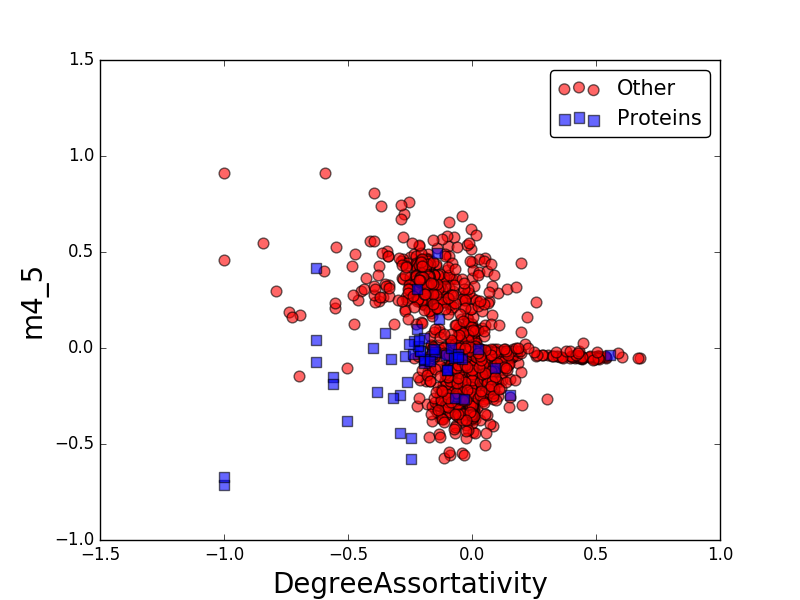
\includegraphics[width=\linewidth]{figs/one_by_many/protein/2d.png}
\caption{Protein interaction.  Average AUC score: 0.689} \label{protein_2d}
\end{subfigure}\hspace*{\fill}
\begin{subfigure}{0.48\textwidth}
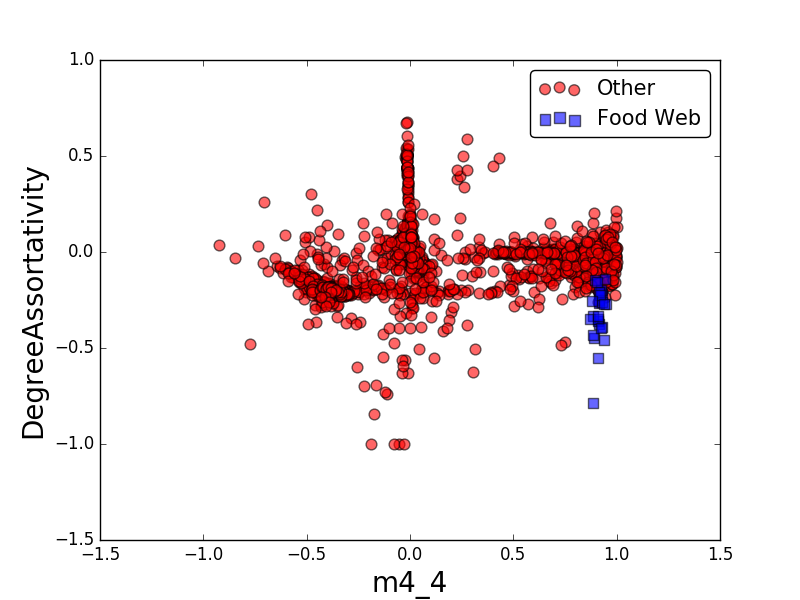
\includegraphics[width=\linewidth]{figs/one_by_many/food_web/2d.png}
\caption{Ecological food web. Average AUC score: 0.804} \label{foodweb_2d}
\end{subfigure}

\medskip
\begin{subfigure}{0.48\textwidth}
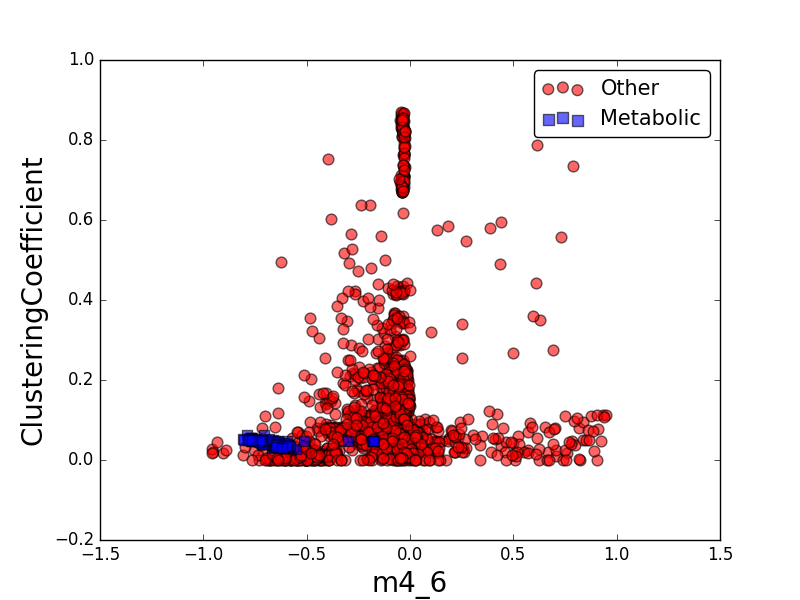
\includegraphics[width=\linewidth]{figs/one_by_many/metabolic/2d.png}
\caption{Metabolic. Average AUC score: 0.94} \label{metabolic_2d}
\end{subfigure}\hspace*{\fill}
\begin{subfigure}{0.48\textwidth}
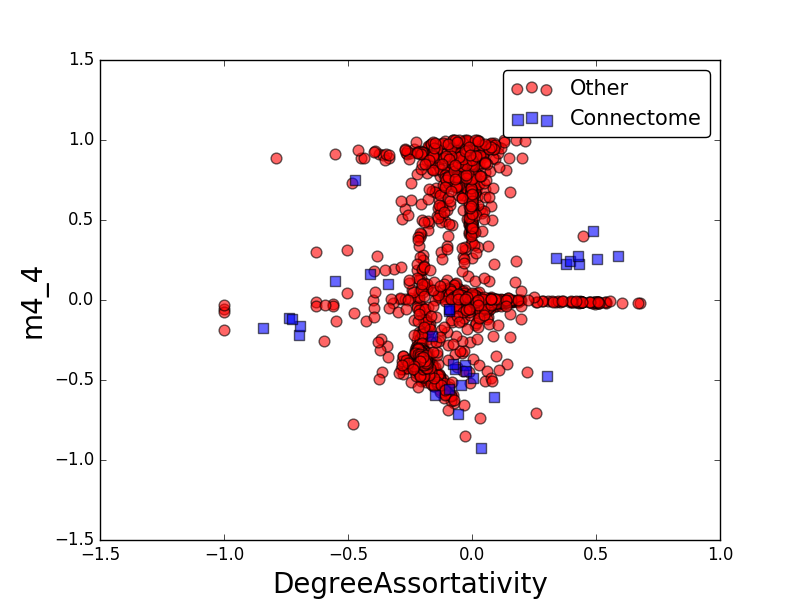
\includegraphics[width=\linewidth]{figs/one_by_many/connectome/2d.png}
\caption{Connectome. Average AUC score: 0.716} \label{connectome_2d}
\end{subfigure}

\medskip
\begin{subfigure}{0.48\textwidth}
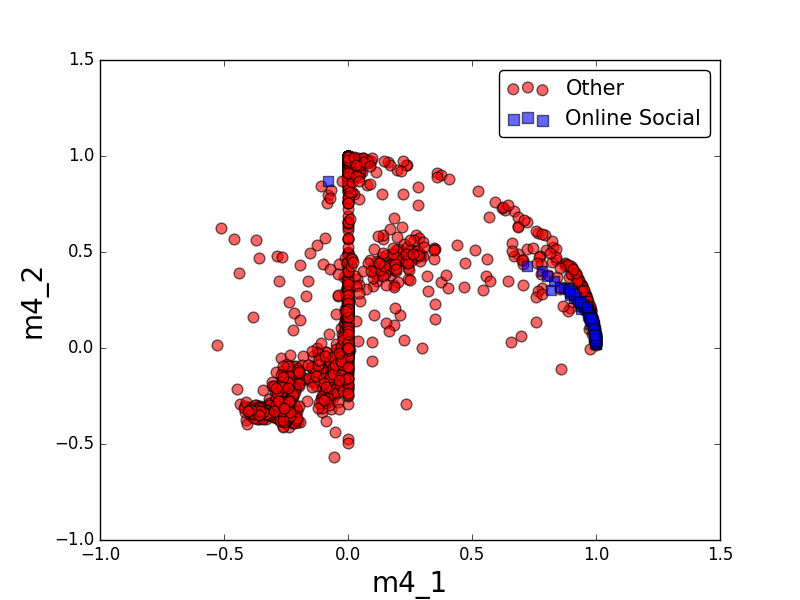
\includegraphics[width=\linewidth]{figs/one_by_many/online_social/2d.png}
\caption{Online social. Average AUC score: 0.94} \label{online_social_2d}
\end{subfigure}\hspace*{\fill}
\begin{subfigure}{0.48\textwidth}
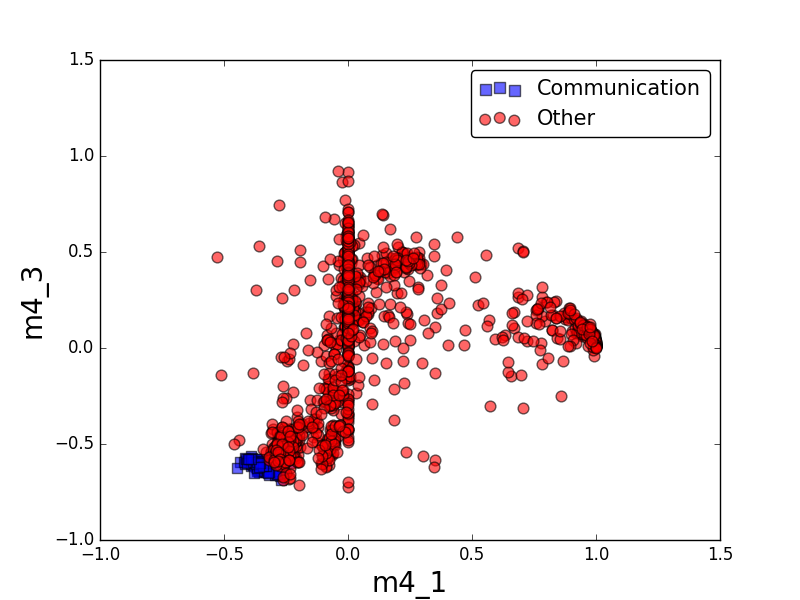
\includegraphics[width=\linewidth]{figs/one_by_many/communication/2d.png}
\caption{Communication. Average AUC score: 0.992} \label{communication_2d}
\end{subfigure}

\caption{2D plots for all representative network sub-domains. X axis corresponds to the most importance feature and y axis the second most important.} \label{2d_figures}
\end{figure}

\begin{figure}[H]
\begin{subfigure}{0.48\textwidth}
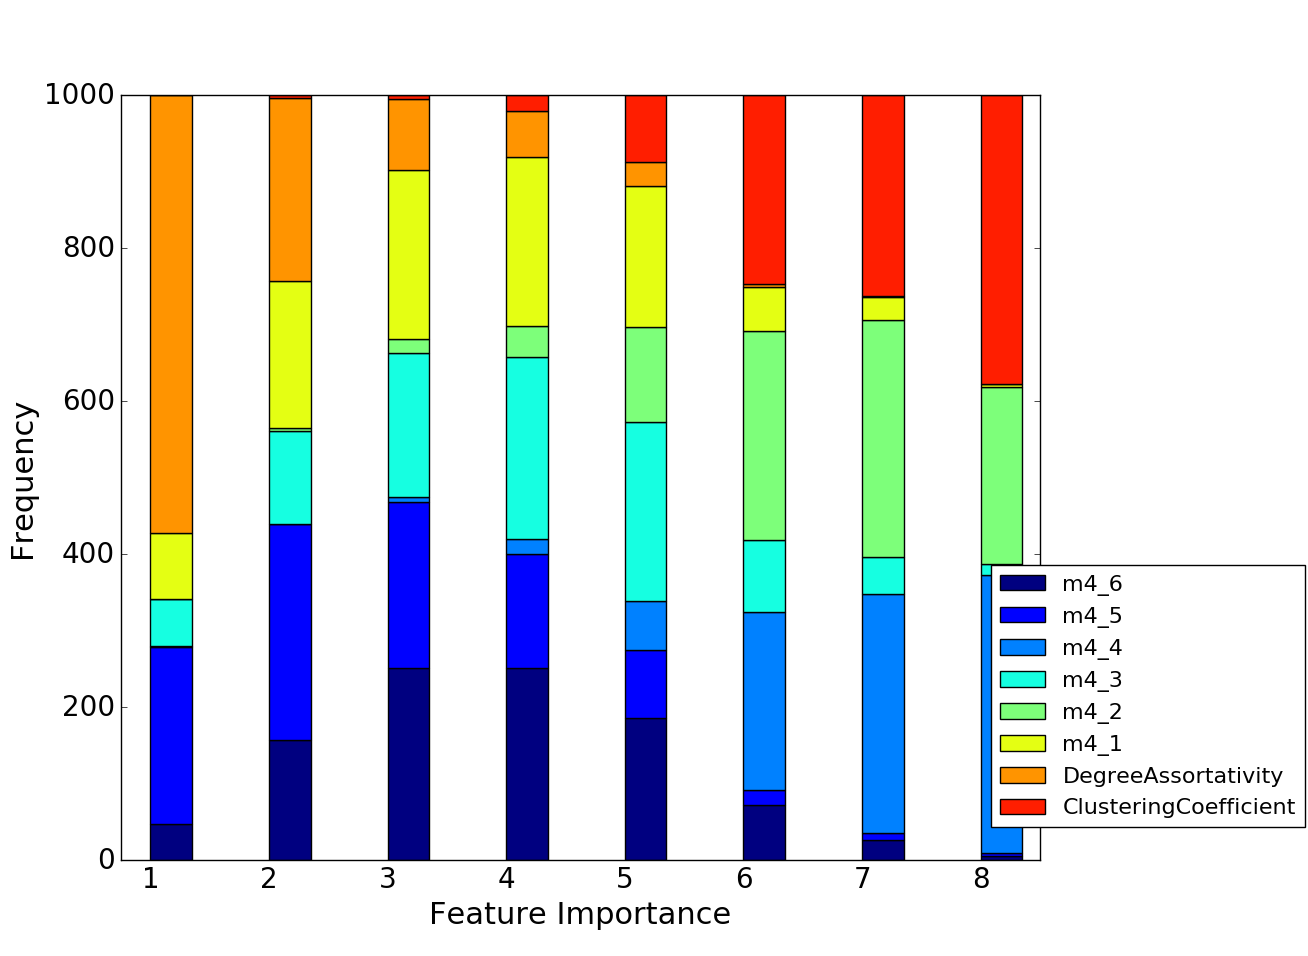
\includegraphics[width=\linewidth]{figs/one_by_many/protein/feature_importance.png}
\caption{Protein interaction.} \label{protein_feature}
\end{subfigure}\hspace*{\fill}
\begin{subfigure}{0.48\textwidth}
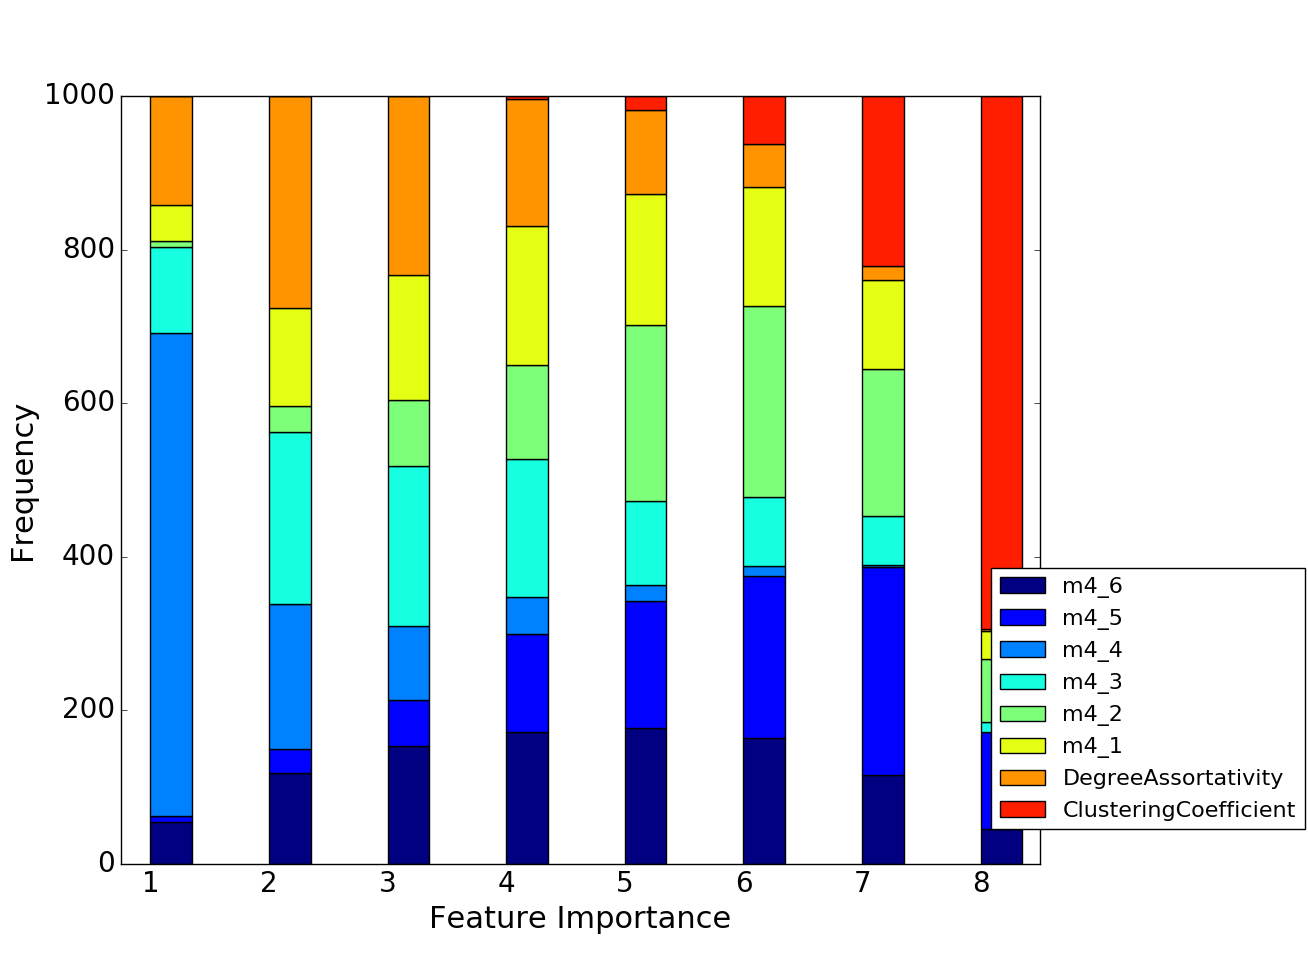
\includegraphics[width=\linewidth]{figs/one_by_many/food_web/feature_importance.png}
\caption{Ecological food web.} \label{foodweb_feature}
\end{subfigure}

\medskip
\begin{subfigure}{0.48\textwidth}
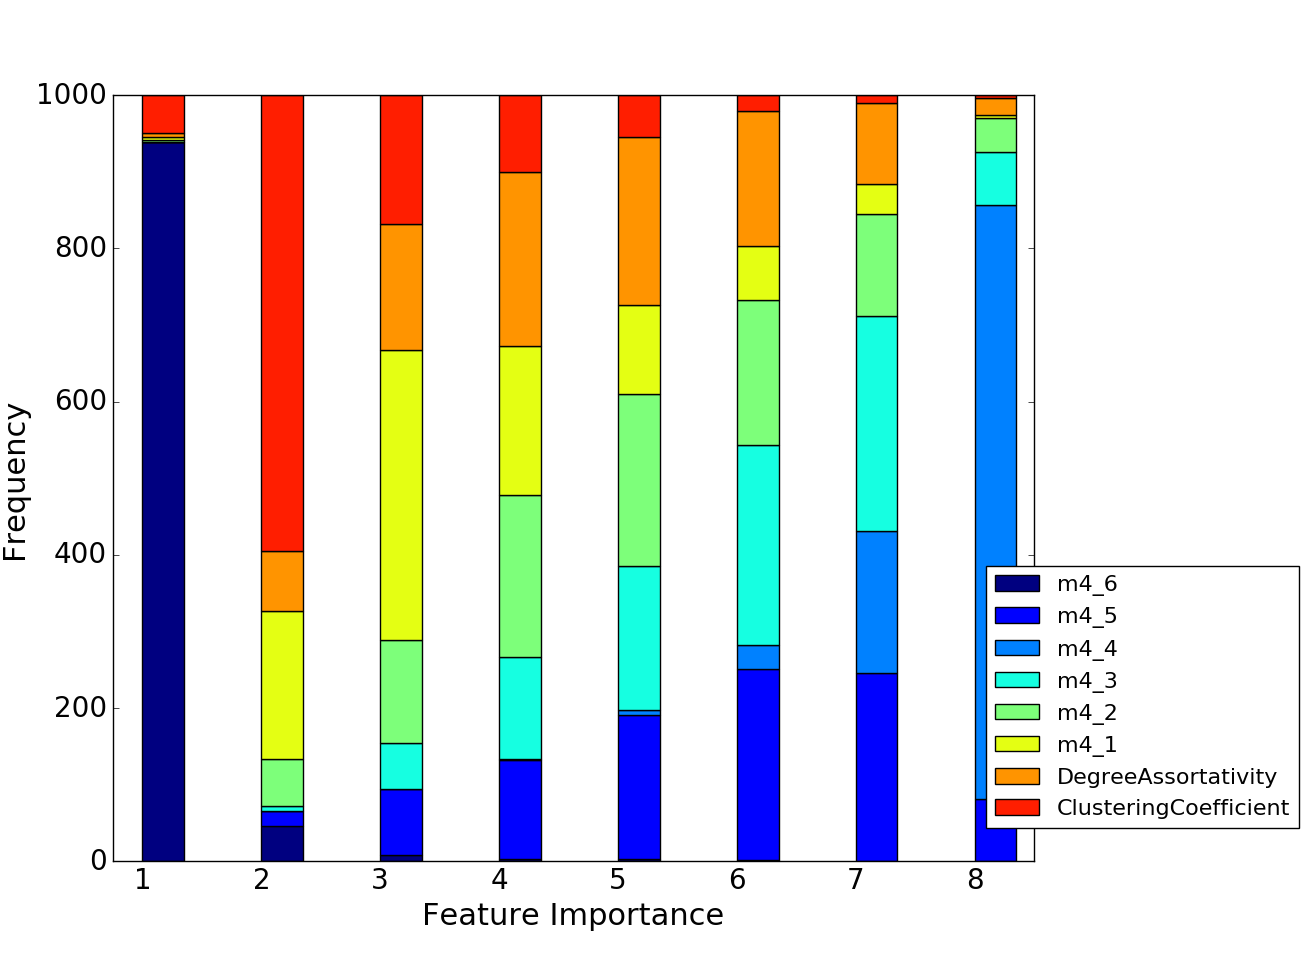
\includegraphics[width=\linewidth]{figs/one_by_many/metabolic/feature_importance.png}
\caption{Metabolic. } \label{metabolic_feature}
\end{subfigure}\hspace*{\fill}
\begin{subfigure}{0.48\textwidth}
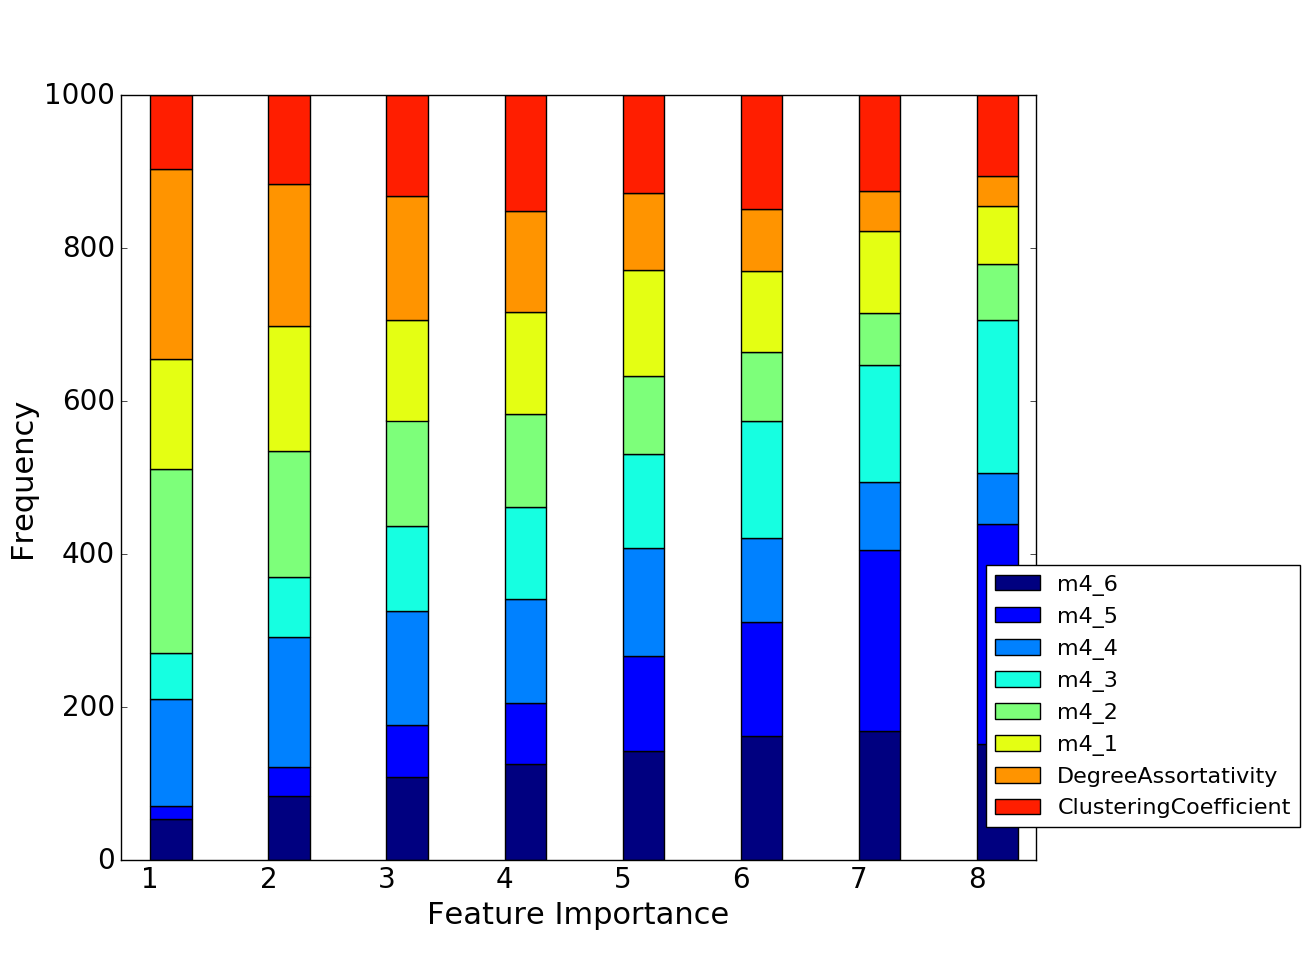
\includegraphics[width=\linewidth]{figs/one_by_many/connectome/feature_importance.png}
\caption{Connectome.} \label{connectome_feature}
\end{subfigure}

\medskip
\begin{subfigure}{0.48\textwidth}
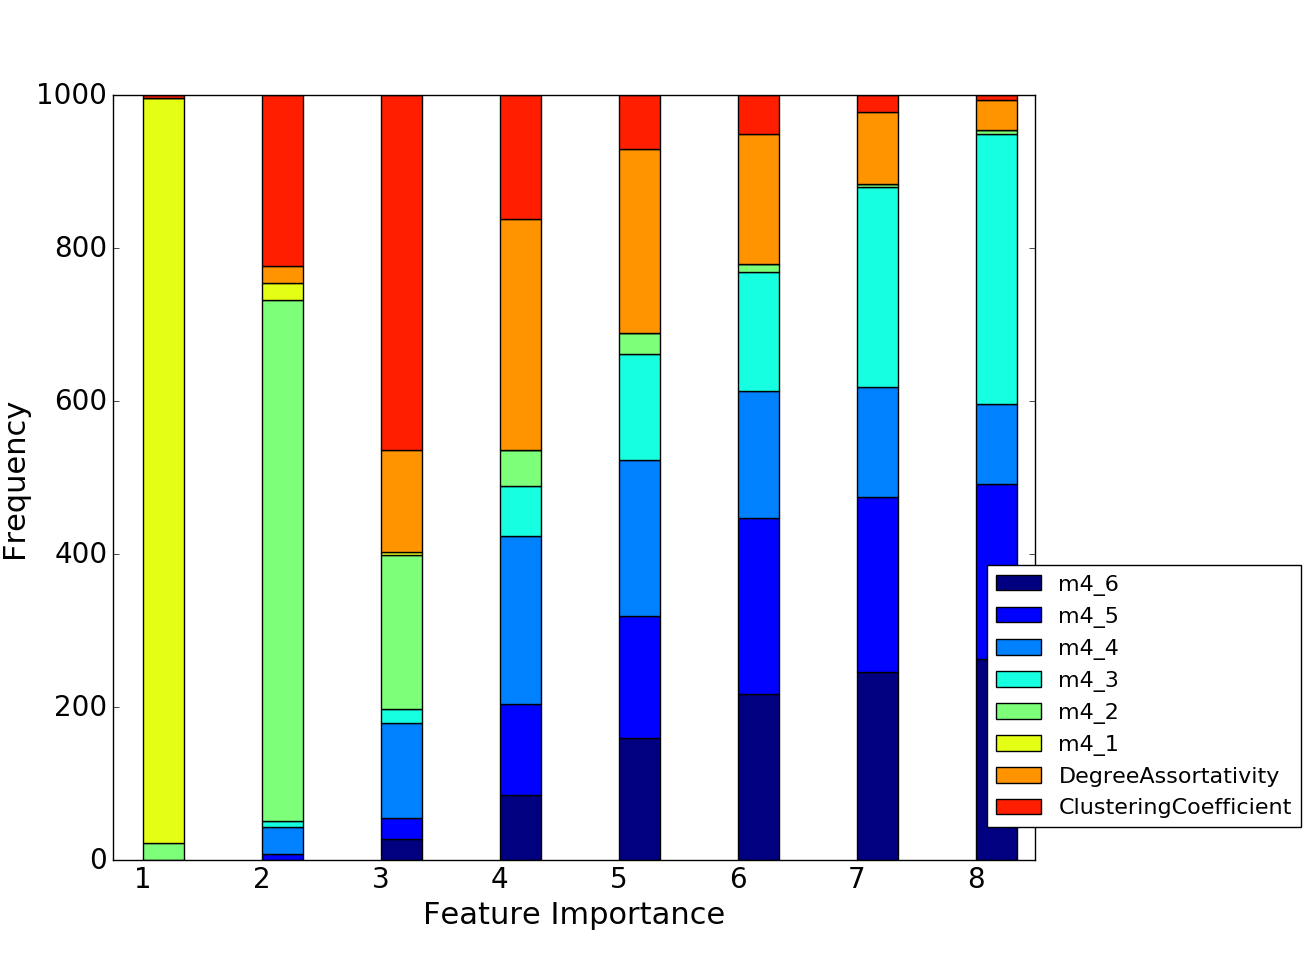
\includegraphics[width=\linewidth]{figs/one_by_many/online_social/feature_importance.png}
\caption{Online social.} \label{online_social_feature}
\end{subfigure}\hspace*{\fill}
\begin{subfigure}{0.48\textwidth}
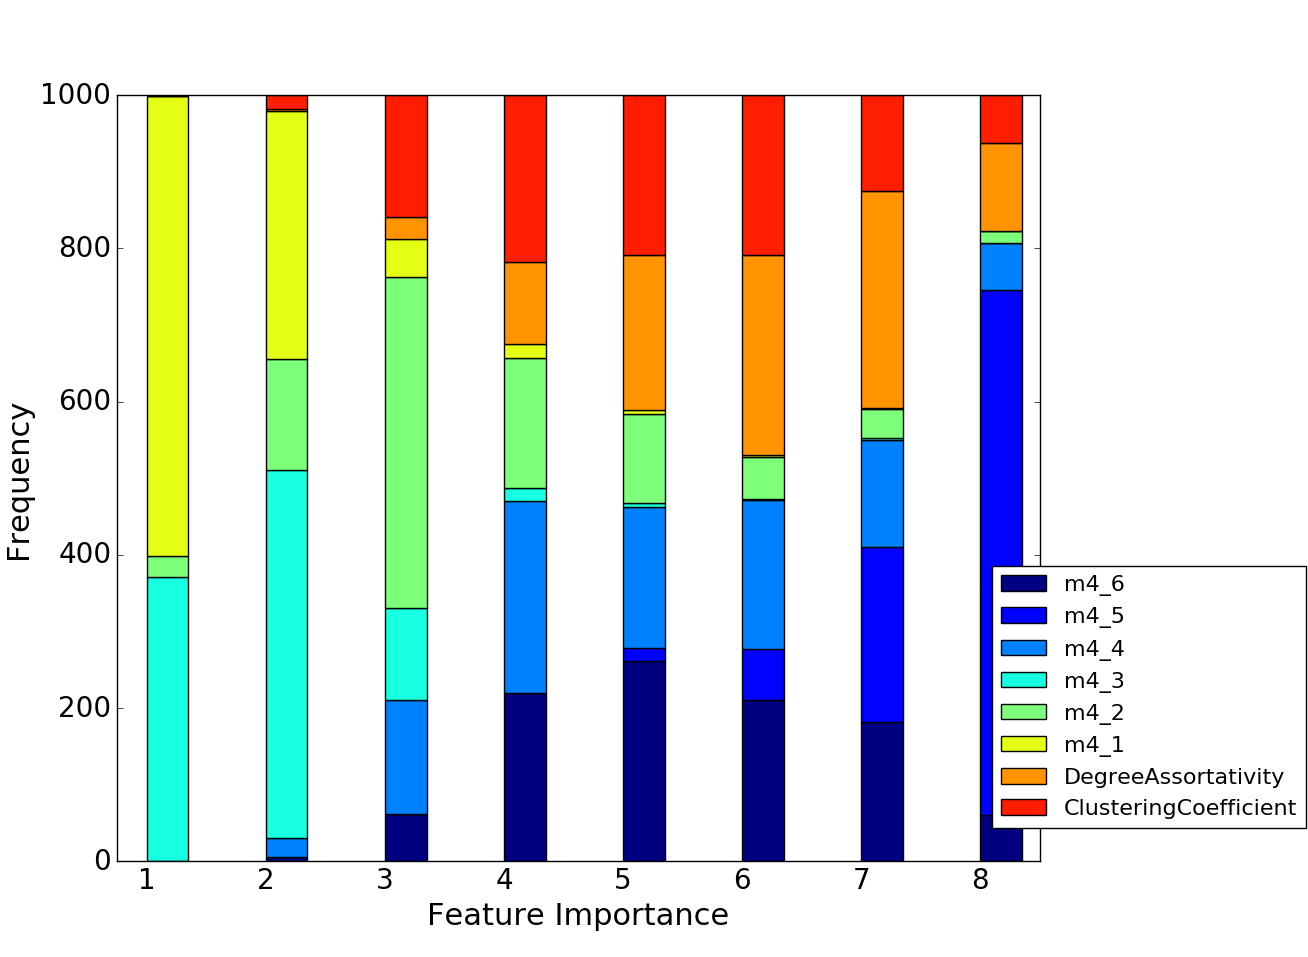
\includegraphics[width=\linewidth]{figs/one_by_many/communication/feature_importance.png}
\caption{Communication.} \label{communication_feature}
\end{subfigure}

\caption{Aggregated rankings of feature importance. The height of a color bar indicates a frequency of the corresponding specific feature being at the rank. The importance decreases along the x-axis} \label{feature_importance_figures}.
\end{figure}


\section{Similarities in Networks of Different Kinds}
Every network belongs to some sort of network domain or sub-domain that usually describes the properties and even structure of a network. As we have seen in the previous section, some networks of selected representative sub-domains exhibit structural uniqueness which makes them stand out among others in the feature space. However we can also observe the overlaps between networks of representative sub-domains and networks of other sub-domains in the Fig. \ref{2d_figures}, which leads to the question we have asked:  \textit{Are there any sets of network categories that are inherently indistinguishable from each other based on network structure?} In this section we explore the structural similarities of different kinds of network domains and sub-domains using machine learning techniques such as random forest and confusion matrix.  

\subsection{Experimental Settings}
We derive structural similarity between network (sub-) domains from a confusion matrix that describes when a random forest classifier makes mistakes and when it does not. However, due to the nature of the classification algorithm and randomly splitting the data into training and testing sets, there involves some randomness in a confusion matrix every time one runs the analysis. Therefore, in order to remove the factor of randomness as much as possible, we run the analysis 1000 times and average the outcomes, namely confusion matrices. Averaging confusion matrices is done element-wise: an element of averaged confusion matrix, say $c$ is defined as $c = \frac{1}{1000}*\sum_{i=1}^{1000} c_i$, where $c_i$ is the corresponding element of an $i$th confusion matrix.

In order to control and compare the impact of class imbalance problem, we use four sampling methods: (i) no-sampling, namely running the analysis on the original data set; (ii) random over-sampling in which minority classes are over-sampled to an extent where all classes have the same number of instances as the largest class; (iii) random under-sampling in which majority classes are under-sampled to an extent where all classes have the same number of instances as the smallest class; (iv) SMOTE in which all minority classes have synthesized new instances so that the number of data points equals to the one of the largest class. A set of features includes, as before, clustering coefficient, degree assortativity and $k = 4$ connected network motifs which result in eight features.
 
 
\subsection{Network Domains} 
We first proceed to work on classification of network domains that include Biological, Social, Informational, Synthetic, Technological and Transportation. Fig.\ref{confusion} shows the aggregated confusion matrices for each of the sampling strategies. In an aggregated confusion matrix, each cell represents the averaged frequency that an instance of class $i$ is classified as class $j$ in 1000 experiments. As the majority classes inherently contain a number of test data points that leads to a larger count in the confusion matrix, there needs to be some normalization so that each class of network domains becomes comparable with others. The normalization in this study is defined as the following: Let $c_{ij}$ be an element in a confusion matrix. We normalize this quantity by a summation of elements in a row $c_{ij}$ belongs to, namely $\sum_{j=1}^N c_{ij}$, where $N$ is the number of network domains. 

The diagonal elements of confusion matrices shown in Fig.\ref{confusion} indicate the correct classifications. In every sampling method, instances of all network domains are relatively classified correctly, which is observable from the colors of the diagonal cells, except Informational networks for which we observe unsuccessful classifications. In spite of the fact that for random-under sampling there are only 26 instances for the training set of each domain, the confusion matrix for the sampling method still exhibits a strong diagonal pattern, which may imply that instances of various network domains are inherently quite separable in the feature space.

Although it is a meaningful result that the instances of network domains may inherently be separable, our focus now moves on to the off-diagonal elements of confusion matrices. In all matrices, a number of instances of Informational networks are classified as other domains, such as Biological, Synthesized and Technological which is observable from elements of a row corresponding to  "true Informational." Also some instances of network domains are classified as Biological networks, observed in elements of a column corresponding to "predicted Biological." 

These pieces of information imply the existence of underlying similarities within network domains. However, it is hard to perceive the structure of inter-domain similarity just by looking at the confusion matrix. Therefore, we construct a network of network domains from a similarity matrix (weighted undirected adjacency matrix) that is constructed based on a confusion matrix that is shown in Fig.\ref{meta_network}. The operation for constructing the similarity matrix based on the normalized confusion matrix is straightforward: we symmetrize the matrix by taking the maximum of two elements in the matrix that are symmetric to each other with respect to a diagonal line. In all cases Biological, Informational and Technological domains are connected with wide edges together, indicating their structural similarities derived from confusion matrices are quite high. From the figure, it appears that there is no "winning" sampling method that produces an outstanding result of a domain network, which means that all of the sampling methods practically produce domain networks that are practically the same.


This analysis which is based on network domains is informative in a sense that it consistently exhibits the well connected group of domains that includes Biological, Informational and Technological. However, each network domain includes sub-domains within itself and these network sub-domains are quite diverse in terms of network's function. For example, neural networks in a brain and ecological food web, both in Biological domain, function very differently. Grouping sub-domains of different functions together as a single category may lose some information local to a specific sub-domain. Therefore, we proceed to analyze the networks on a more fine-grained setting, namely using network sub-domains as the class label in classification tasks.
 

\begin{figure}[H]
\begin{subfigure}{0.48\textwidth}
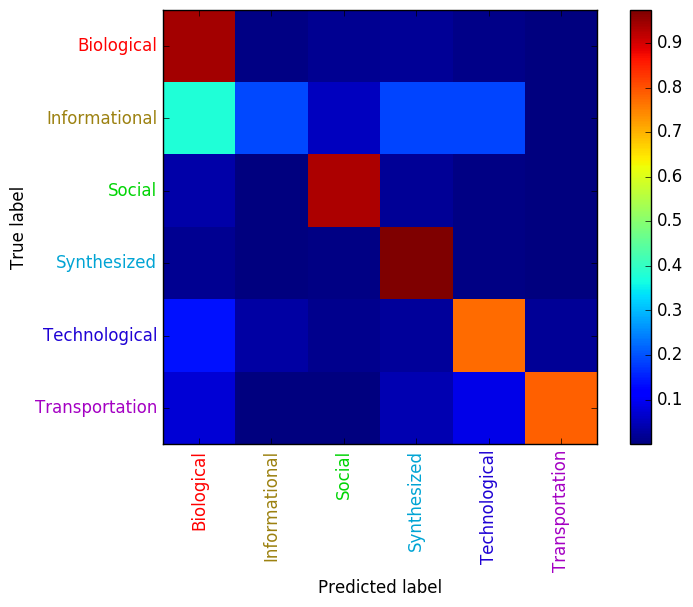
\includegraphics[width=\linewidth]{figs/similarity/Domain/None/confusion_None.png}
\caption{No sampling.} \label{no_confusion}
\end{subfigure}\hspace*{\fill}
\begin{subfigure}{0.48\textwidth}
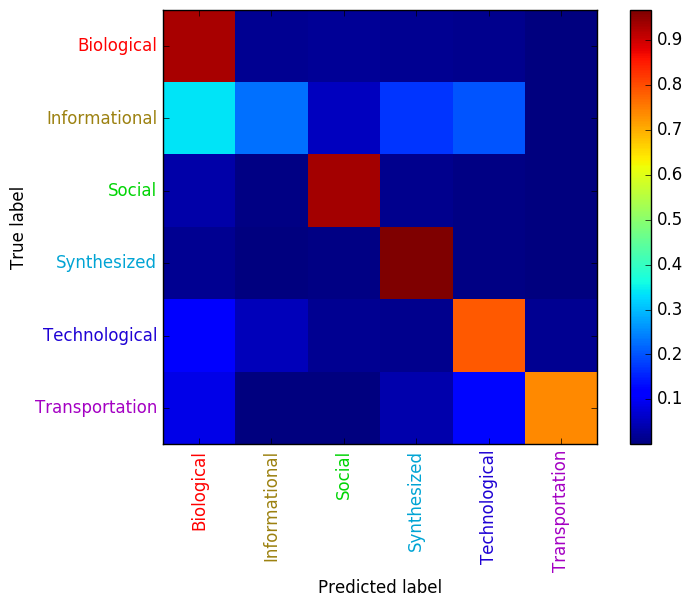
\includegraphics[width=\linewidth]{figs/similarity/Domain/RandomOver/confusion_RandomOver.png}
\caption{Random over-sampling. } \label{random_over_confusion}
\end{subfigure}

\medskip
\begin{subfigure}{0.48\textwidth}
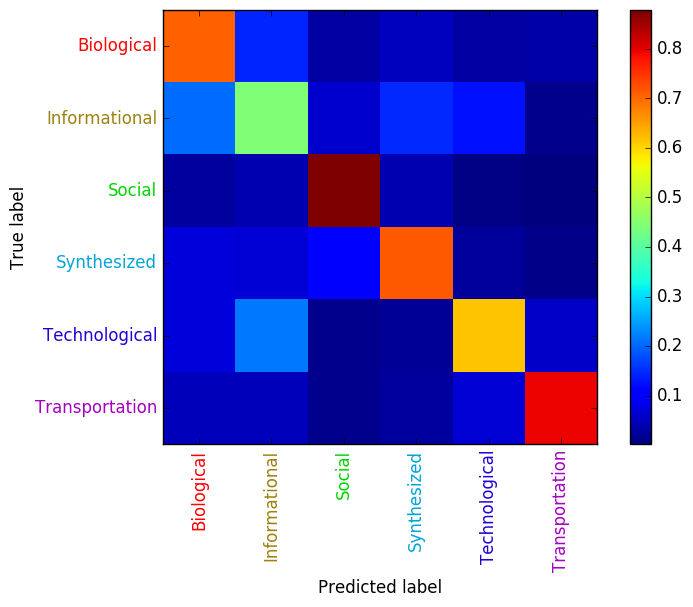
\includegraphics[width=\linewidth]{figs/similarity/Domain/RandomUnder_26/confusion_RandomUnder.png}
\caption{Random under-sampling. } \label{random_under_confusion}
\end{subfigure}\hspace*{\fill}
\begin{subfigure}{0.48\textwidth}
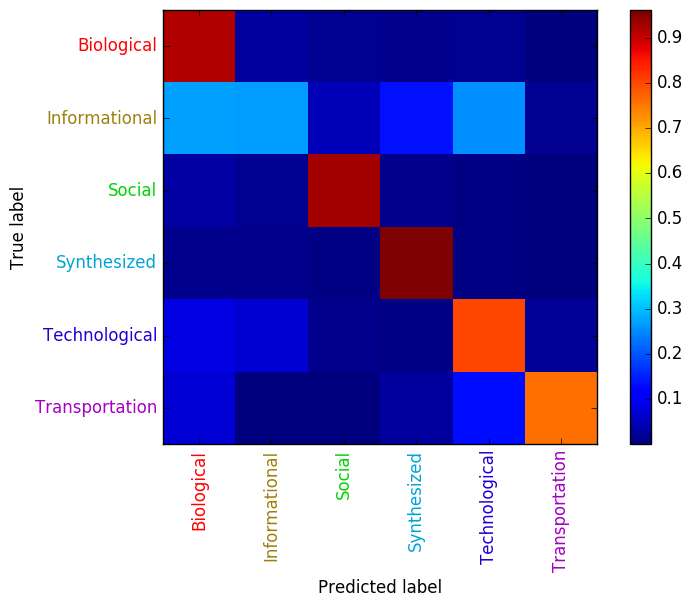
\includegraphics[width=\linewidth]{figs/similarity/Domain/SMOTE/confusion_SMOTE.png}
\caption{SMOTE.} \label{smote_confusion}
\end{subfigure}
\
\caption{Confusion matrices for each of the sampling strategy. The color of each cell represents a count value normalized by the sum of all counts in a row the cell belongs to. Our similarity measurement is based on this normalized value of a confusion matrix.} \label{confusion}
\end{figure}

\begin{figure}[H]
\begin{subfigure}{0.48\textwidth}
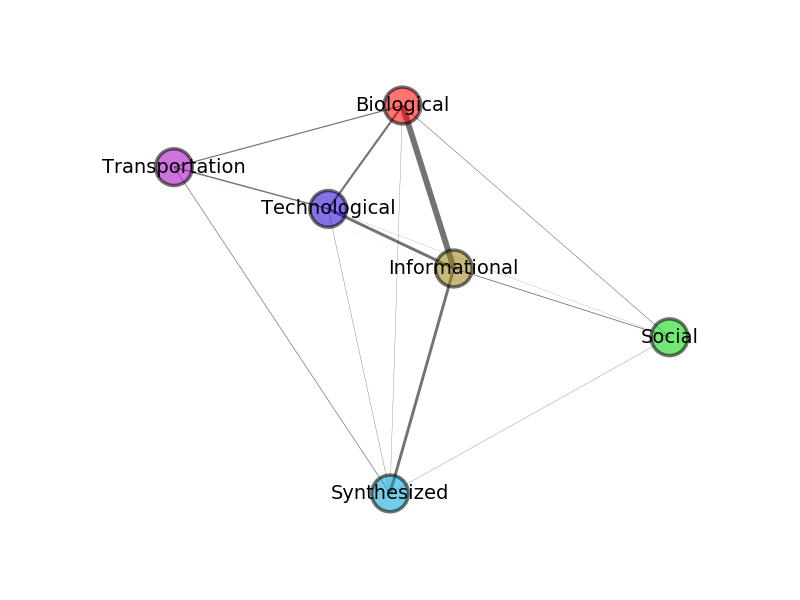
\includegraphics[width=\linewidth]{figs/similarity/Domain/None/g.png}
\caption{No sampling} \label{no_graph}
\end{subfigure}\hspace*{\fill}
\begin{subfigure}{0.48\textwidth}
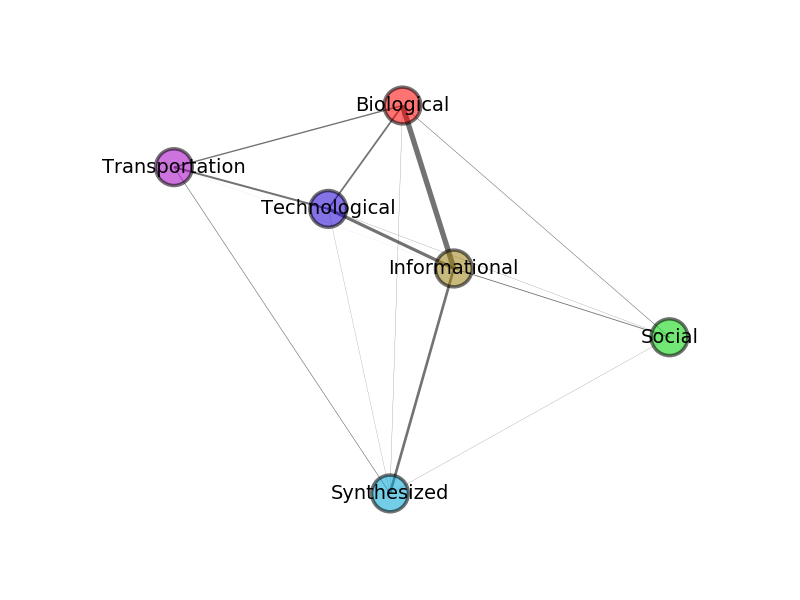
\includegraphics[width=\linewidth]{figs/similarity/Domain/RandomOver/g.png}
\caption{Random over-sampling.} \label{random_over_graph}
\end{subfigure}

\medskip
\begin{subfigure}{0.48\textwidth}
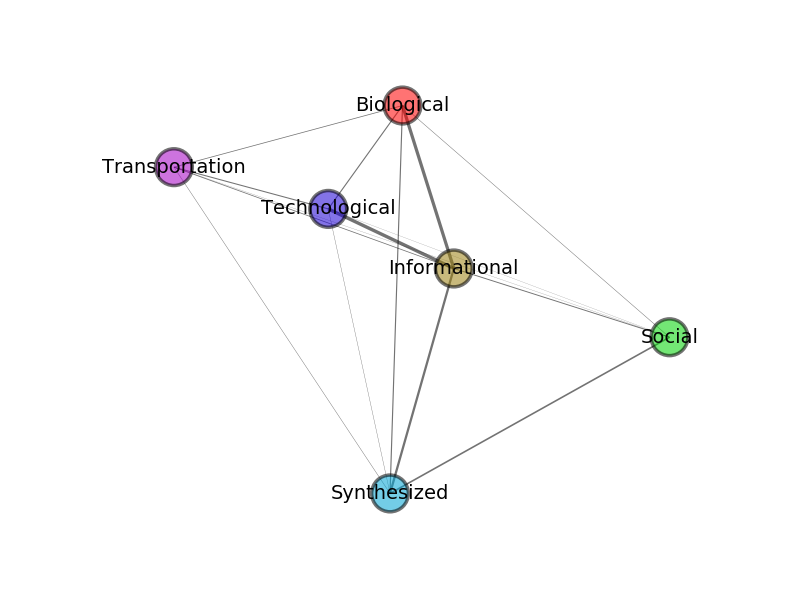
\includegraphics[width=\linewidth]{figs/similarity/Domain/RandomUnder_26/g.png}
\caption{Random under-sampling.} \label{random_under_graph}
\end{subfigure}\hspace*{\fill}
\begin{subfigure}{0.48\textwidth}
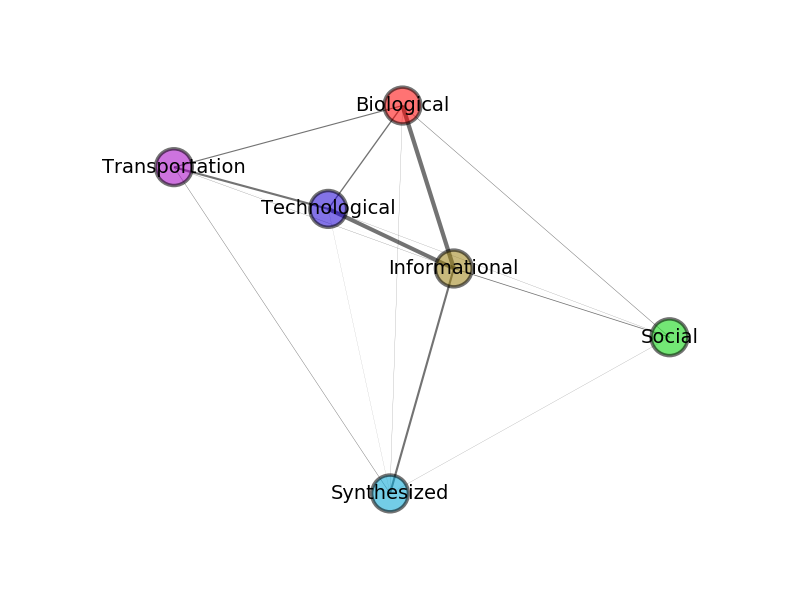
\includegraphics[width=\linewidth]{figs/similarity/Domain/SMOTE/g.png}
\caption{SMOTE.} \label{smote_graph}
\end{subfigure}
\
\caption{Domain networks for different sampling strategies. The widths of edges are proportional to the magnitude of a value in a symmetrized, normalized confusion matrix. Biological, Informational and Technological domains are well connected in all cases.} \label{meta_network}
\end{figure}


\subsection{Network Sub-domains}
Here we continue the same analysis as we have done in the previous section, but using network sub-domains as class labels for classification tasks.
Although in total we have 33 network sub-domains as shown in Fig. \ref{sub_dist}, some sub-domains have only few instances, which makes it infeasible to proceed to classification tasks as they involve train-test split of data and SMOTE assumes a training set to have enough amount of instances for selecting $k$ nearest neighbors. Therefore we first exclude sub-domains that the number of instances within themselves are less than seven, which enables us to split the training and test sets in the ratio of $7:3$ while keeping the class distribution in both sets the same and SMOTE to successfully find $k=3$ nearest neighbors for any sub-domain. This filtering results in 22 network sub-domains for this analysis\footnote{The excluded network subdomains are: Language, Relatedness, Legal, Commerce, Recommendations, Collaboration, Fiction, Relationships, Email, Power grid and Airport.}. 

Same as the previous setting for network domain, we run classification tasks 1000 times for each sampling method, aggregate, normalize and symmetrize the resulting confusion matrices. Figure \ref{confusion_sub} shows the aggregated confusion matrices for each sampling method in which we can observe that all of the confusion matrices exhibit the diagonal pattern, an indication of underlying separability of network sub-domains. Note that, however, some sub-domains such as bayesian, web graph, offline social, water distribution and software dependency, are often not classified correctly which may be due to the few instances and/or the fact that network structures of their instances are actually quite similar to the ones of other sub-domains. It is obvious to notice that the aggregated confusion matrix for random under-sampling displays fewer white cells within itself, meaning that under this sampling method the classifier confused a number of sub-domains with other sub-domains.

In order to visualize the underlying similarities within network sub-domain, we again construct networks of sub-domains based on a weighted undirected adjacency matrix derived from aggregated confusion matrices, shown in Fig.\ref{meta_network}. From this figure, we can observe that the network domain is not necessarily a good indicator of sub-domain clustering: informational networks including web graph, bayesian and peer to peer network and biological networks, such as metabolic, fungal, food web, etc. are not clustered together, meaning that we do not observe the sub-domains having the same color forming a community together. This could be attributed to the fact that some network domains, such as biological networks, entail a broad spectrum of network sub-domains within itself whose instances are drastically different in terms of the physical size of the things nodes represent (from cells to animals) and the process of networks (from chemical reactions to prey-predator relationships). 

Then the question is: \textit{What could be a good indicator of similarity in networks of different kinds?} In order to answer this question, we first need to discover the communities of subdomain networks which are groups of nodes within which the weighted edge density is high, but between which the weighted edge density is low.

Fig.\ref{meta_network_community} shows the networks of sub-domains on which the colors of nodes correspond to the community membership found by a community detection algorithm proposed by Clauset \textit{et al.} \cite{CNMAlgorithm}. We have used an implementation of the modified version of this algorithm for weighted network that is available in Python-igraph as a method \texttt{community\_fastgreedy()} \cite{igraph}. From Fig.\ref{meta_network_community}, one may notice that the community structure across different sampling methods is almost consistent, meaning that the certain groups of sub-domains are always in the same community.  For instance, for all sampling methods, offline social, connectome and affiliation networks are in the same community. 

Some network sub-domains, however, change the community membership for some subdomain networks. For instance, online social network and forest fire model networks join the community of off-line social network for no sampling, random-over sampling and random-under sampling method, but joins the community of software dependency (red color) for SMOTE sampling. This variation of community membership across all subdomain networks could be attributed to the effect of each sampling method on decision surfaces a classifier builds for classification. For instance, decision surfaces built by a classifier under the random under-sampling strategy should be simple shape-wise since the training set is very sparse in terms of the number of data points. On the other hand, decision surfaces built by a classifier for random over-sampling should be more toward complicated shape-wise and lead to over-fitting as the number of data points for training is larger and duplicated points force the classifier to adjust itself to those points. Therefore this variation of decision surfaces may lead some data points to be classified differently for different sampling method, which ultimately leads to the variation of community memberships.


\begin{figure}[H]
	\begin{subfigure}{0.48\textwidth}
	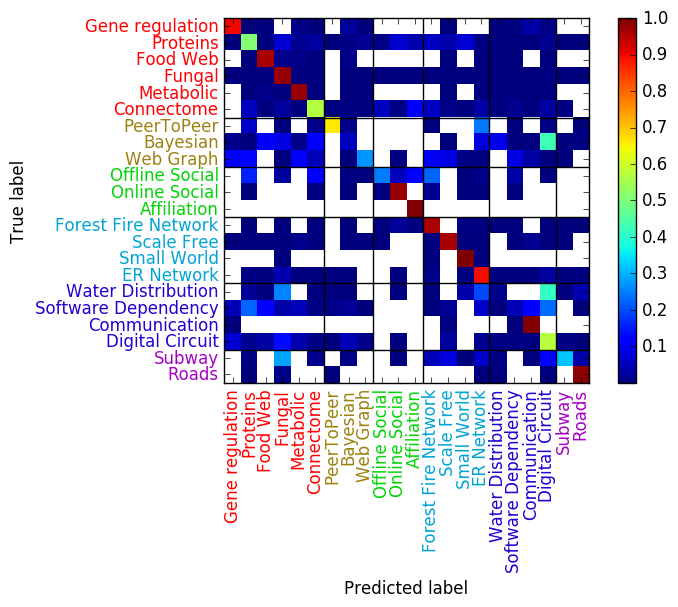
\includegraphics[width=\linewidth]{figs/similarity/SubDomain/None/confusion_sub_None.png}
	\caption{No sampling. } \label{no_confusion_sub}
	\end{subfigure}\hspace*{\fill}
	\begin{subfigure}{0.48\textwidth}
	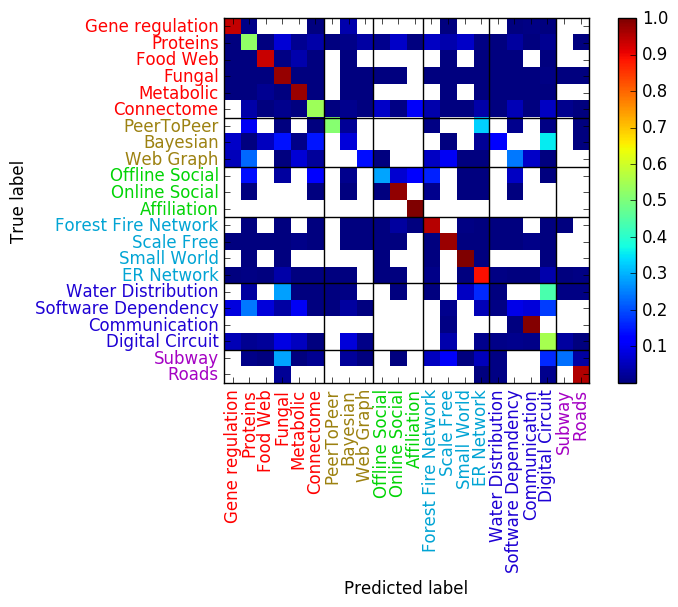
\includegraphics[width=\linewidth]{figs/similarity/SubDomain/RandomOver/confusion_sub_RandomOver.png}
	\caption{Random over-sampling. } \label{random_over_confusion_sub}
	\end{subfigure}
	
	\medskip
	\begin{subfigure}{0.48\textwidth}
	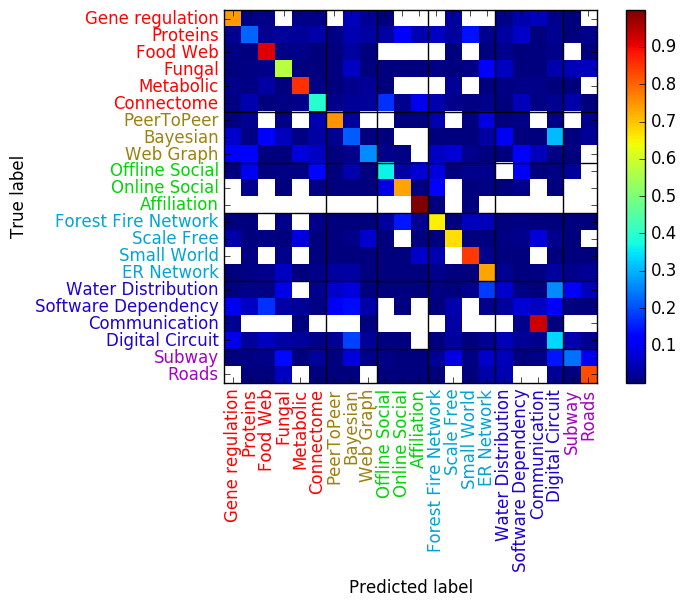
\includegraphics[width=\linewidth]{figs/similarity/SubDomain/RandomUnder_all5/confusion_sub_RandomUnder.png}
	\caption{Random under-sampling. } \label{random_under_confusion_sub}
	\end{subfigure}\hspace*{\fill}
	\begin{subfigure}{0.48\textwidth}
	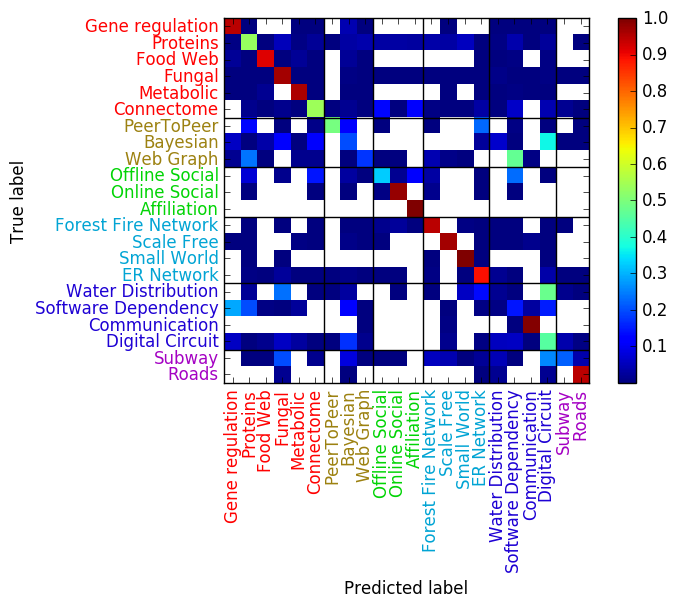
\includegraphics[width=\linewidth]{figs/similarity/SubDomain/SMOTE/confusion_sub_SMOTE.png}
	\caption{SMOTE. } \label{smote_confusion_sub}
	\end{subfigure}
\
\caption{Confusion matrices for each of the sampling method. The white cells in confusion matrices indicate zero occurrence of corresponding classifications: sub-domain $i$ is misclassified as sub-domain $j$. The color of each cell represents a count value normalized by the sum of all counts in a row the cell belongs to. Our similarity measurement is based on the normalized value of a confusion matrix shown in above. Lines within confusion matrices indicate the separations of network domains.} \label{confusion_sub}
\end{figure}

\begin{figure}[H]
	\begin{subfigure}{0.48\textwidth}
	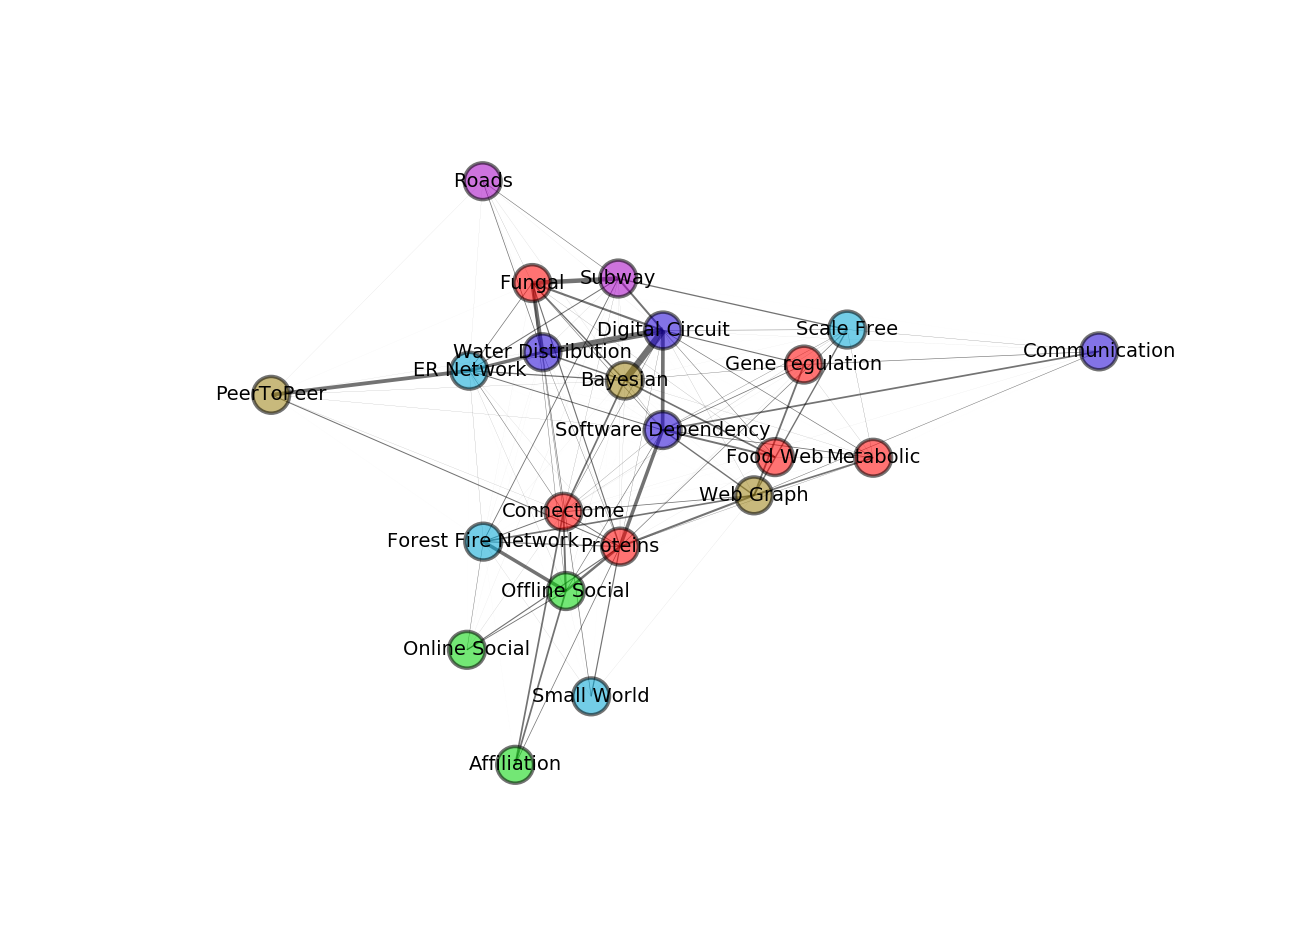
\includegraphics[width=\linewidth]{figs/similarity/SubDomain/None/g.png}
	\caption{subdomain network based on no sampling.} \label{no_graph_sub_original}
	\end{subfigure}\hspace*{\fill}
	\begin{subfigure}{0.48\textwidth}
	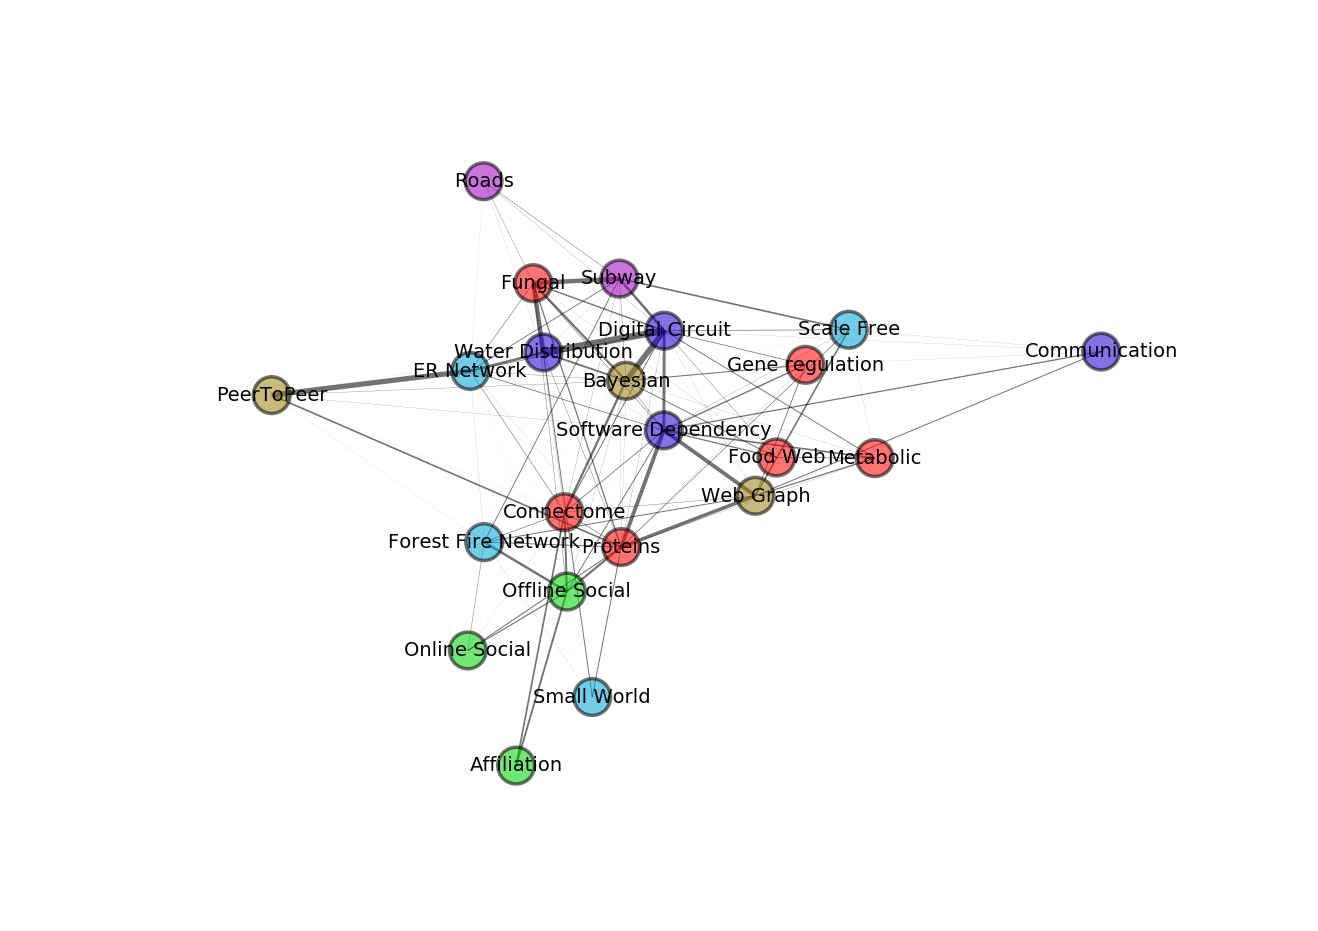
\includegraphics[width=\linewidth]{figs/similarity/SubDomain/RandomOver/g.png}
	\caption{subdomain network based on random over-sampling.} \label{random_over_graph_sub_original}
	\end{subfigure}
	
	\medskip
	\begin{subfigure}{0.48\textwidth}
	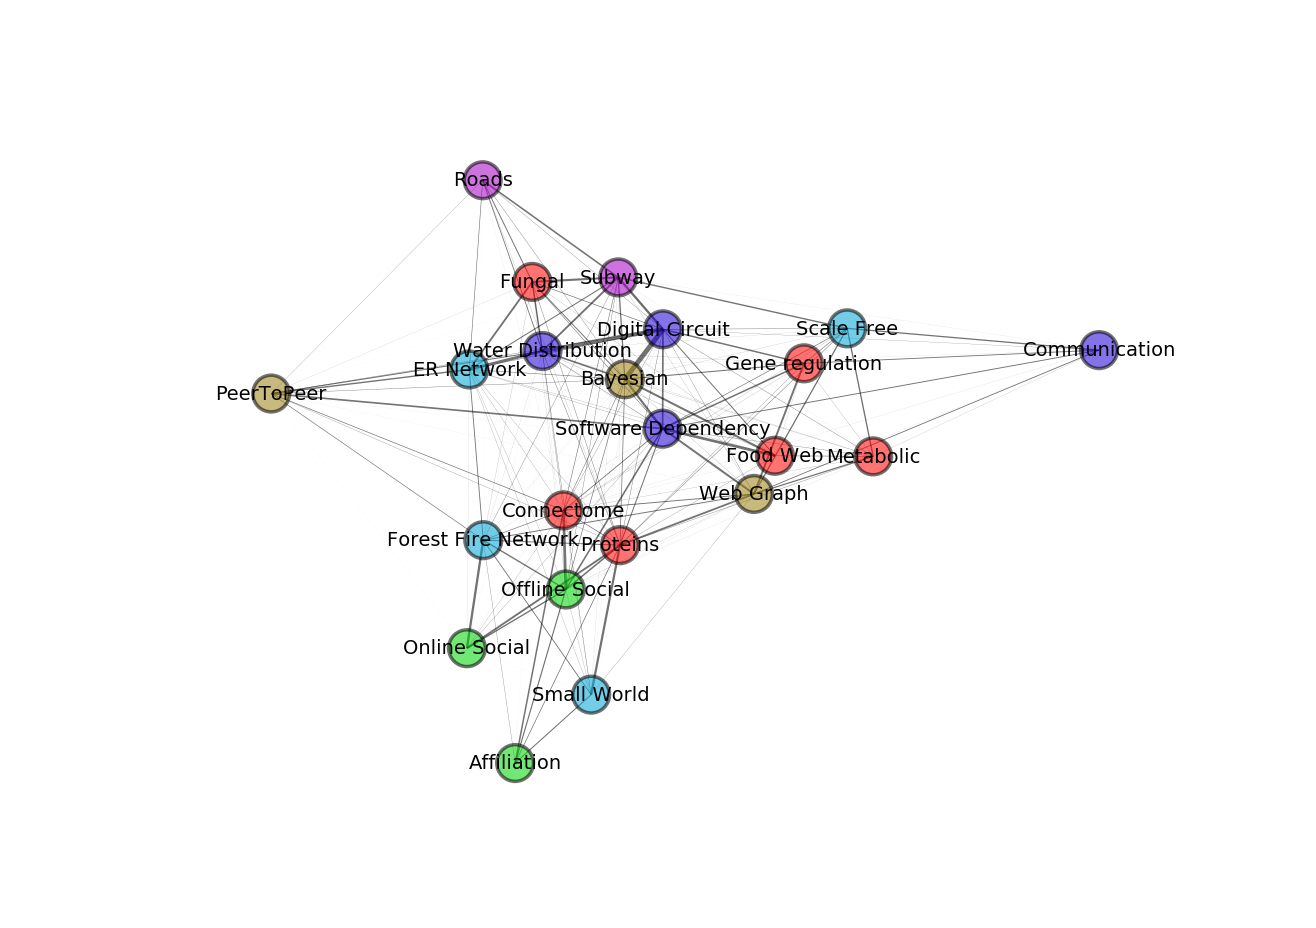
\includegraphics[width=\linewidth]{figs/similarity/SubDomain/RandomUnder_all5/g.png}
	\caption{subdomain network based on random under-sampling.} \label{random_under_graph_sub_original}
	\end{subfigure}\hspace*{\fill}
	\begin{subfigure}{0.48\textwidth}
	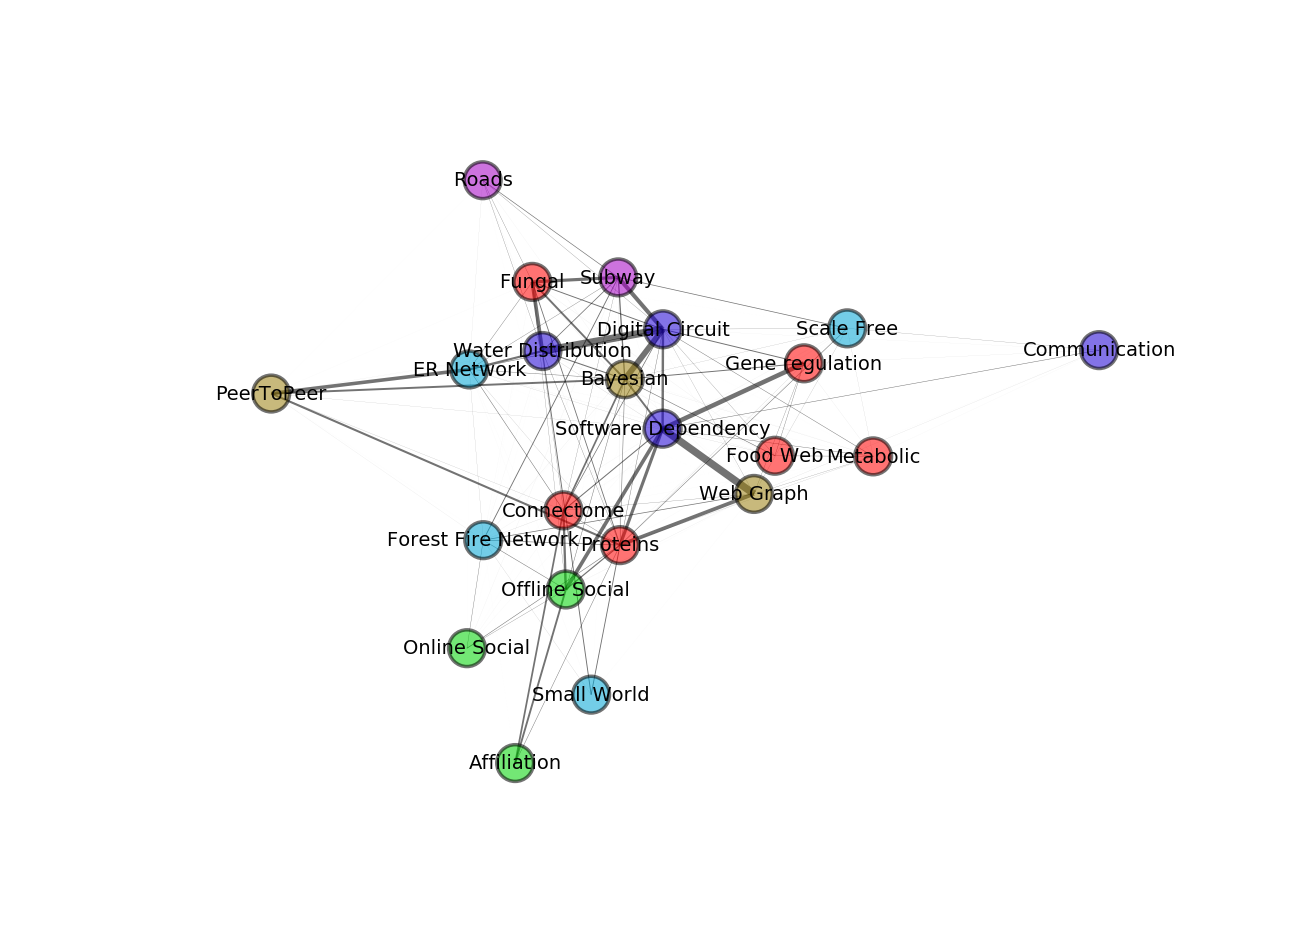
\includegraphics[width=\linewidth]{figs/similarity/SubDomain/SMOTE/g.png}
	\caption{subdomain network based on SMOTE.} \label{smote_graph_sub_original}
	\end{subfigure}
\
\caption{The networks of sub-domains. The color of each node corresponds to a domain the sub-domain (node) belongs to and width of each edge corresponds to the similarity of sub-domains derived from the aggregated confusion matrix.} \label{meta_network}
\end{figure}

\begin{figure}[H]
	\begin{subfigure}{0.48\textwidth}
	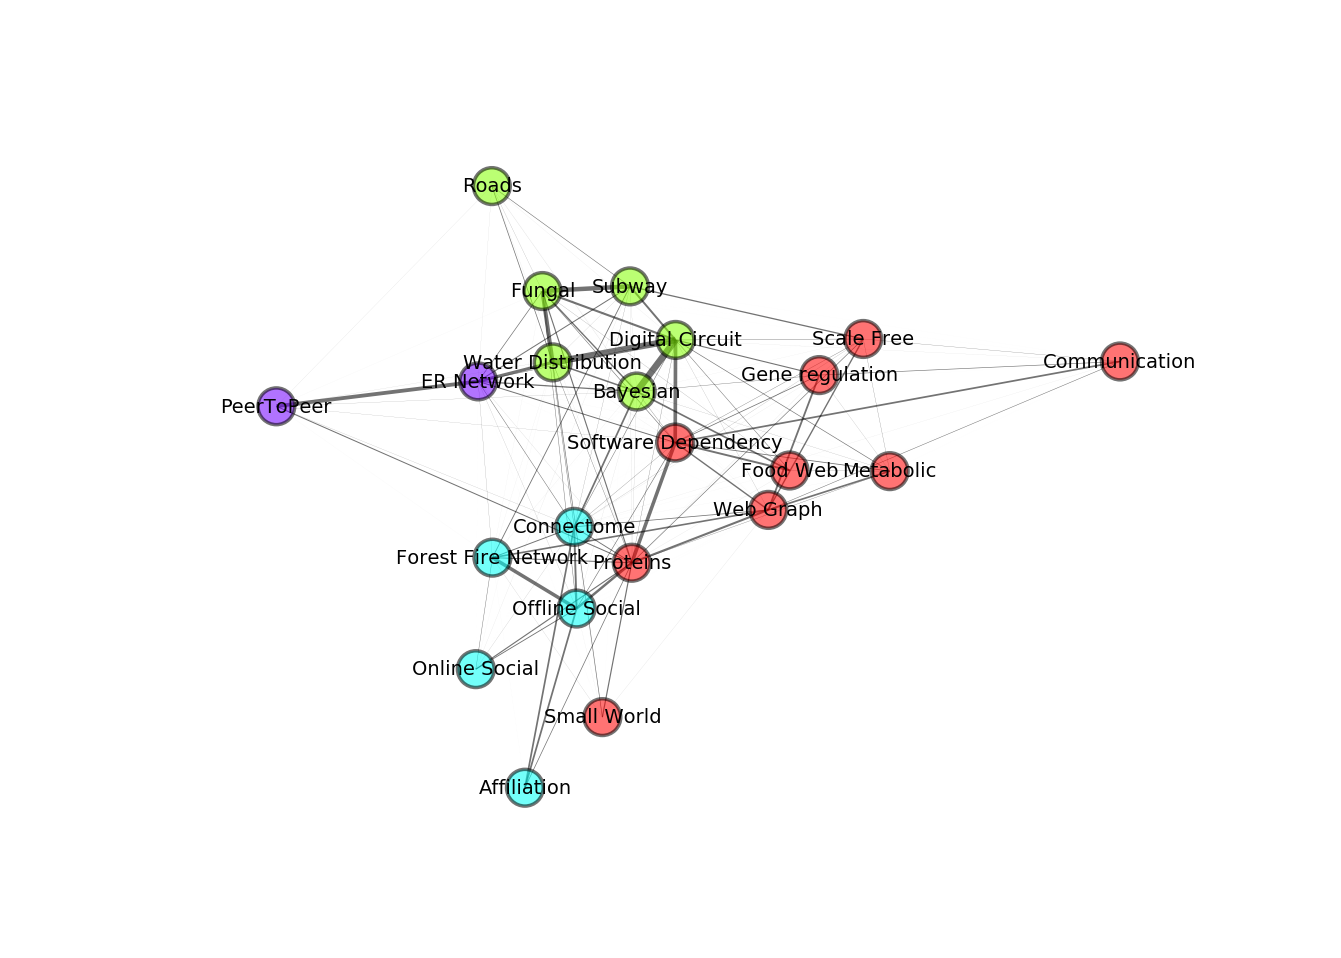
\includegraphics[width=\linewidth]{figs/similarity/SubDomain/None/g_community.png}
	\caption{subdomain network based on no sampling. The number of communities is $4$.} \label{no_graph_sub_community}
	\end{subfigure}\hspace*{\fill}
	\begin{subfigure}{0.48\textwidth}
	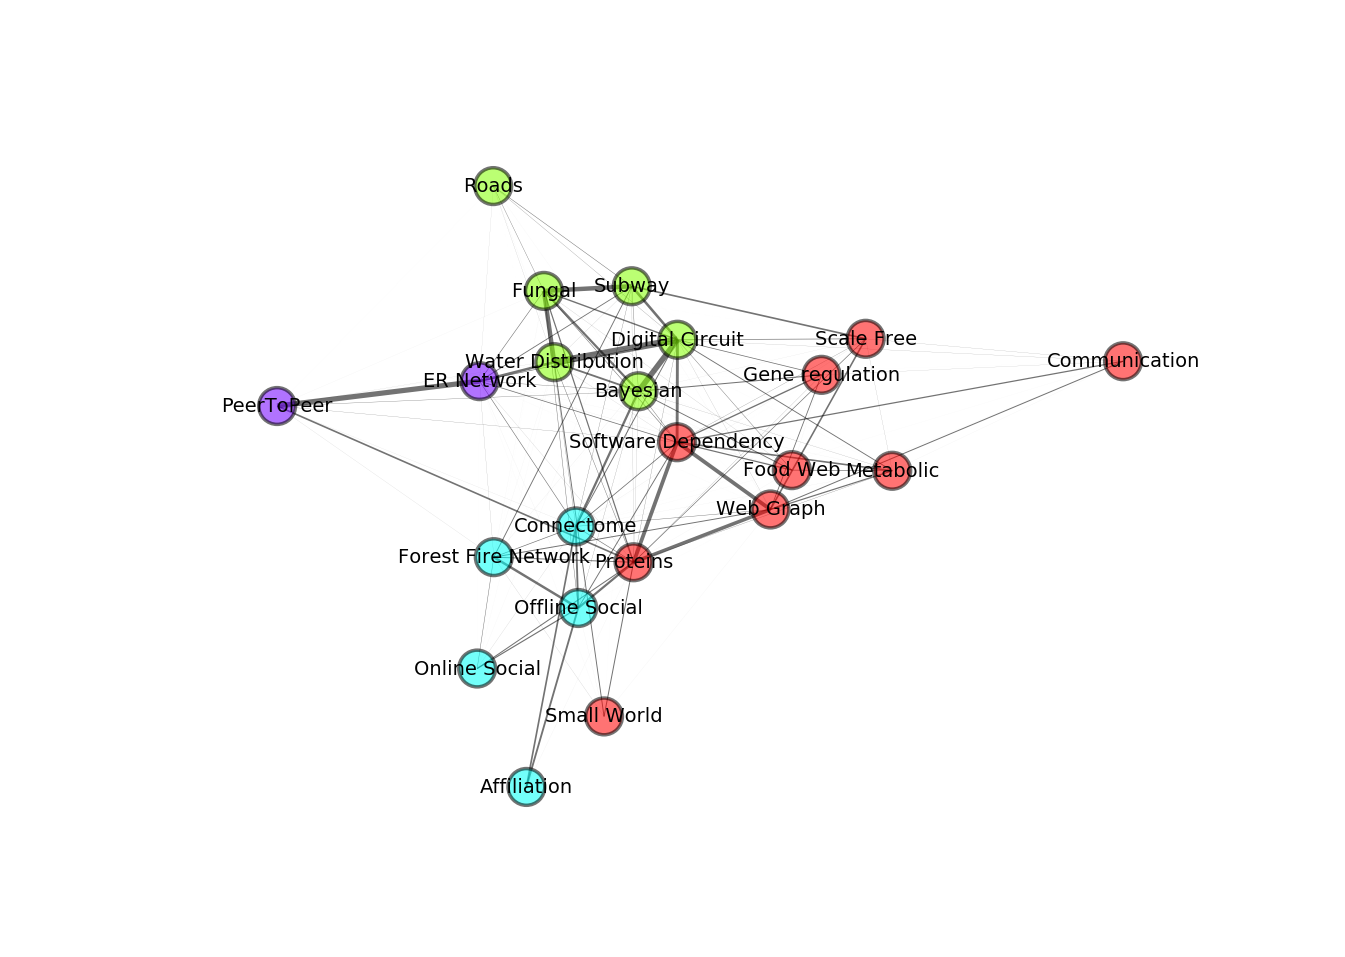
\includegraphics[width=\linewidth]{figs/similarity/SubDomain/RandomOver/g_community.png}
	\caption{subdomain network based on random over-sampling sampling.  The number of communities is $4$.} \label{random_over_graph_sub_community}
	\end{subfigure}
	
	\medskip
	\begin{subfigure}{0.48\textwidth}
	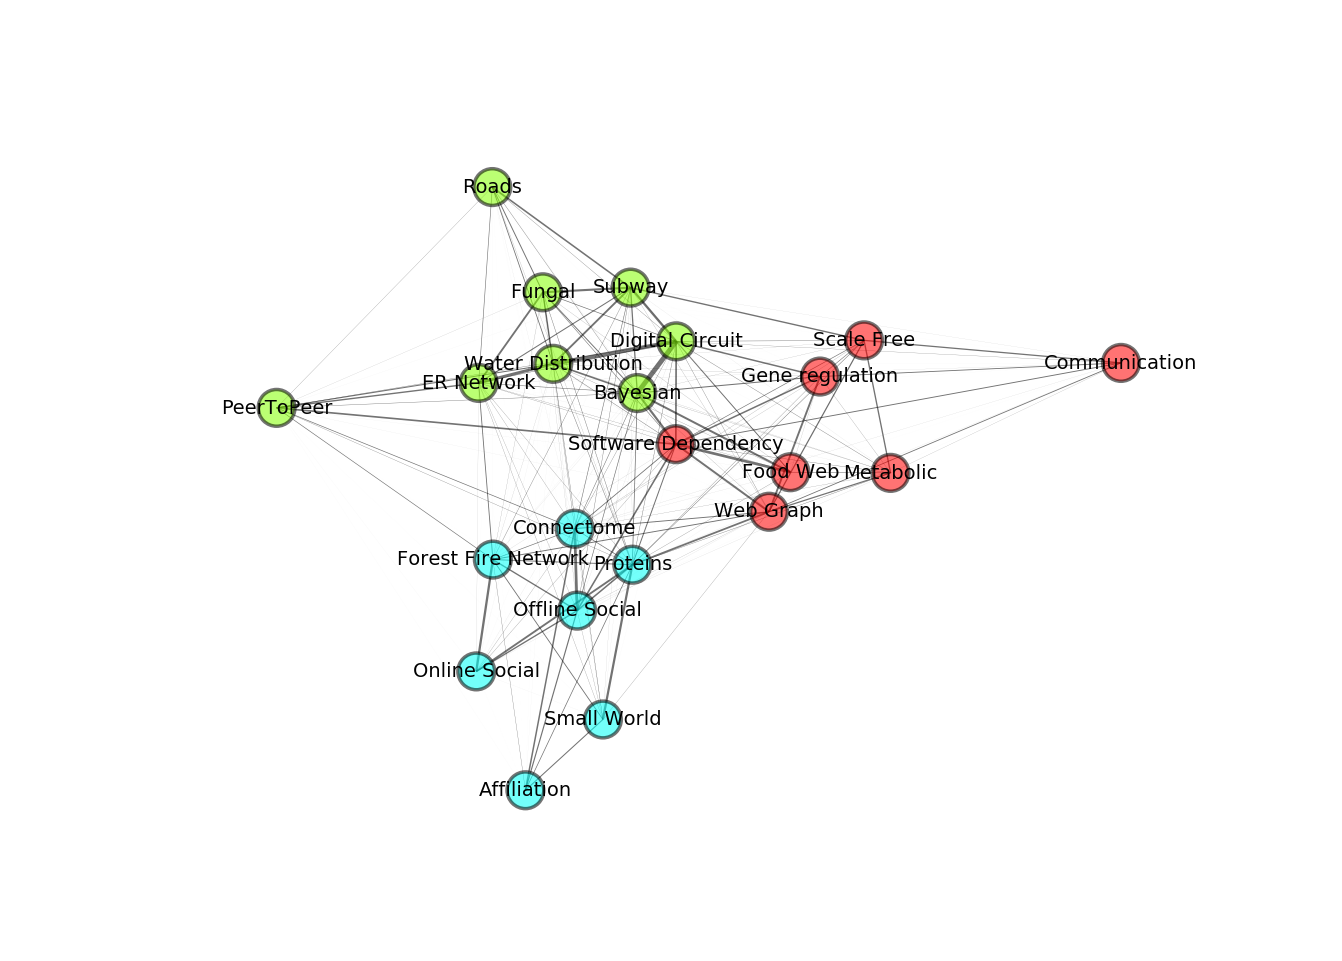
\includegraphics[width=\linewidth]{figs/similarity/SubDomain/RandomUnder_all5/g_community.png}
	\caption{subdomain network based on random under-sampling.  The number of communities is $3$.} \label{random_under_graph_sub_community}
	\end{subfigure}\hspace*{\fill}
	\begin{subfigure}{0.48\textwidth}
	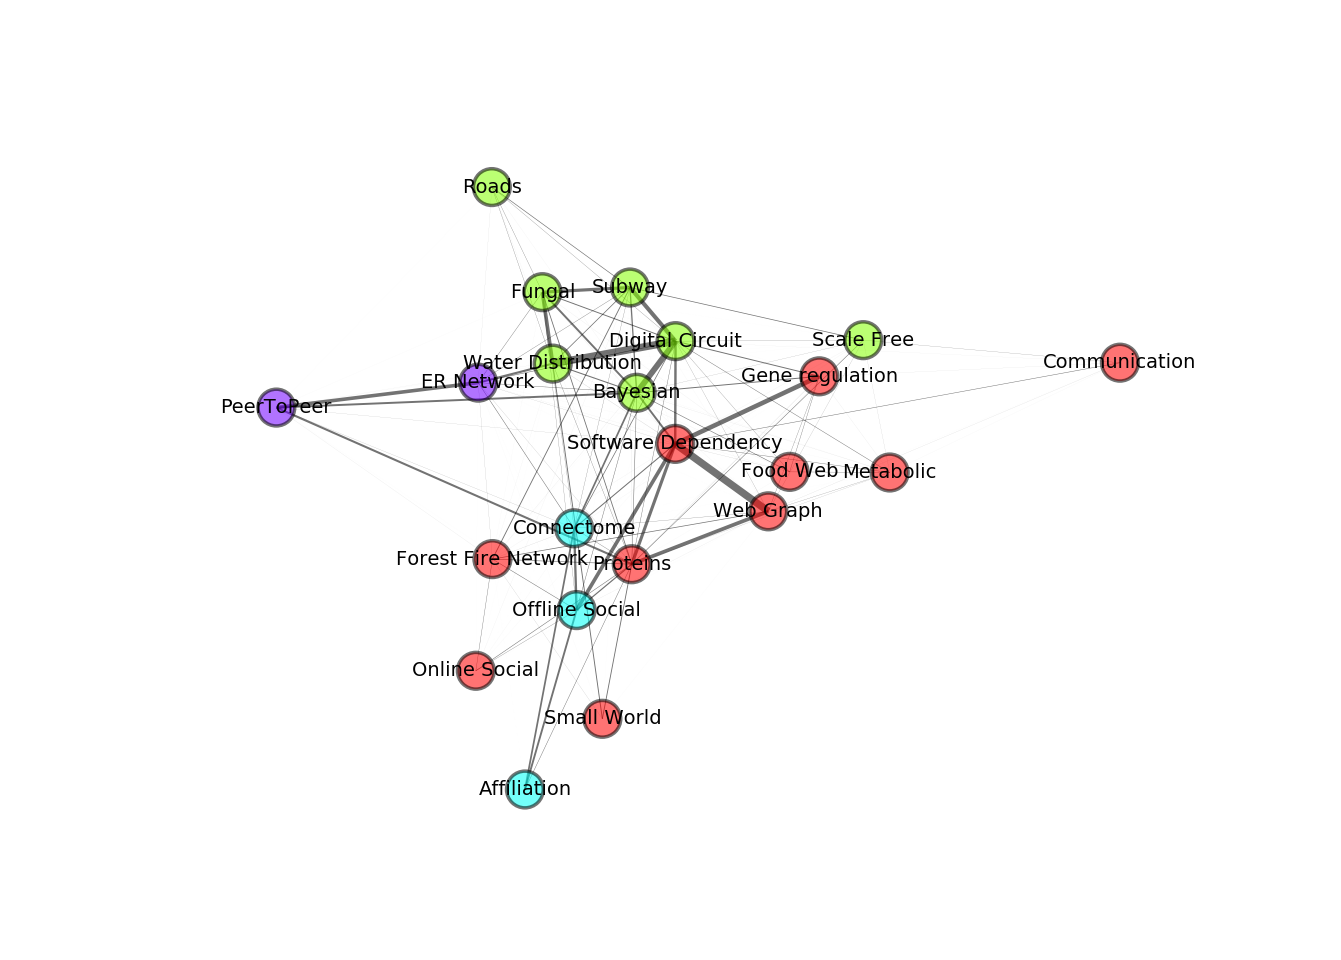
\includegraphics[width=\linewidth]{figs/similarity/SubDomain/SMOTE/g_community.png}
	\caption{subdomain network based on SMOTE.  The number of communities is $4$.} \label{SMOTE_graph_sub_community}
	\end{subfigure}
\
\caption{The networks of sub-domains with community labelings. The color of a node now corresponds to a community found by the algorithm and width of each edge corresponds to the similarity of sub-domains derived from the aggregated confusion matrix.} \label{meta_network_community}
\end{figure}



In order to facilitate analyzing the variation of community memberships, we have constructed a matrix, shown in Fig.\ref{community_overlaps} in which the frequency that two sub-domain share the same community membership corresponds to the color intensity. For instance offline social, connectome and affiliation networks are assigned to the same community four times. From this figure, one may notice that there appears to be three groups of sub-domains that are consistently assigned to the same community. The first one is a community of social networks including online and offline social networks as well as affiliation network and forest fire model with an exception of connectome, namely brain networks. This grouping of social networks could be attributed to the same underlying process, namely forest fire process: on online social networks, namely Facebook networks, one becomes a friend with someone, and finds other friends on the person's friend list, sends them friend requests and recursively continues the process; on off-line social networks, a person introduces his/her friends to you, they also introduce their friends to you and the process recursively continues. The possible explanations why we observe connectome being in the same community as such social networks are as follows: (i) the lack of feature or dimension in the feature space that distinguishes brain networks from social networks; (ii) the underlying generative mechanism of brain network is actually similar to that of social networks. As far as we know, however, there is no previous study investigating commonality of processes of both social and brain networks. Therefore it is reasonable to speculate here that we lacked a set of distinguishing features for connectome, which resulted in the clustering of the network with social networks.

The second group of sub-domains corresponds to the networks that have been claimed to have the power-law degree distribution which include scale-free network, metabolic network, web graph, etc. and some of these networks have been conjectured to grow according to a mechanism called preferential attachment. In this network generative process, newly added nodes in a network, for example newly created web page or software package, tend to connect to the popular or high-degree nodes, i.e. popular web sites or widely used software packages. The third and last group of sub-domains is the network of "flow" that includes electrical signal (digital circuit), information (bayesian), water (water distribution), nutrient (fungal), people/trains (subway) and cars (road).  Also, if we look at the subdomain networks, digital circuit and bayesian networks are always tightly connected together. This may be due to the fact that they are both an input-output network as well as being a flow network. The rest of the flow networks have another common property, that is, physical embedding of the network. These networks have a strong constraint of the physical limitation. For instance, it is almost impossible for a node in a physically embedded network to have a thousand connections upon it.

From these communities of sub-domains, one could hypothesize an idea that explains what governs the structure of complex networks: functionality, constraint and growing mechanism of networks may play an important role of the formation of a specific network structure. As we have seen, the sub-domains of networks that have the similar functionality, constraint or growing mechanism exhibit the similar structural pattern which is captured in confusion matrices and also communities of networks. However, there seems to be a case where we do not know why a network sub-domain is in a community and how the hypothesis would explain this: connectome, or brain network shares the same community with social networks. If our hypothesis is correct, then brain networks should have either the same function, constraint or growing mechanism as social networks. As far as we know, there is no study which compares connectome and social networks in terms of network structure and explains the similarity of their function, constraint and generative mechanism. One possible direction to take would be finding a set of features for which those sub-domains have similar values and investigate a possible generative process which yields networks having such structural features.

Although there are some exceptional cases, our findings from this experiment provide some supporting evidence that the network structure may be influenced by the underlying function, constraint and growing mechanism of the network.


\begin{figure}[ht]
		\begin{center}
		\vspace{0.5cm}
		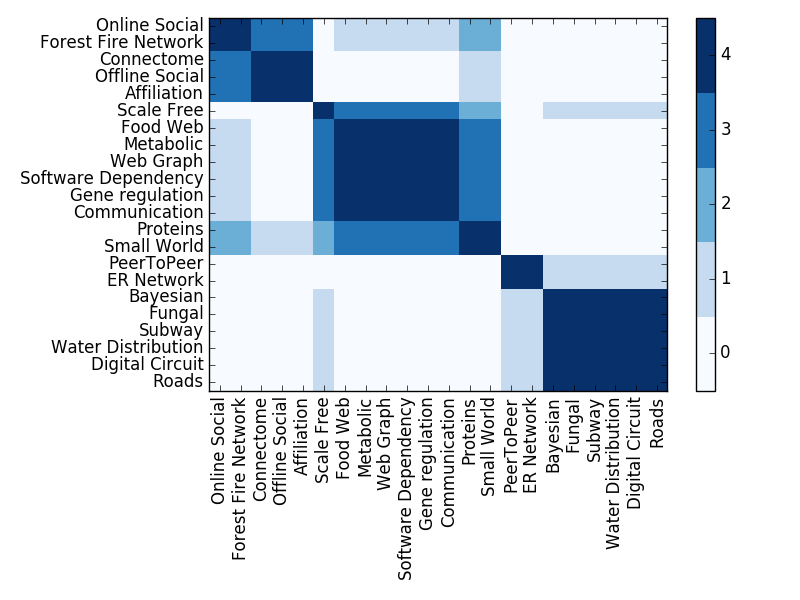
\includegraphics[clip,width=12cm,height = 9cm]{figs/overlaps.png}
		\vspace{0.5cm}
		\caption{Overlaps of community memberships. The intensity of color for each cell in the matrix indicates the frequency of two sub-domains being in the same community.  There are three groups of sub-domains that almost constantly share the community membership: (i) community of social networks including online social, forest fire model, offline social, and so on; (ii) community of networks claimed to have a power-law degree distribution including scale-free network, metabolic network, web graph, etc. with some exceptions such as small world network; (iii) community of networks that are physically embedded, having an input-output function or containing some sort of flow on the network, which include road, digital circuit and fungal networks.}
		\label{community_overlaps}
 		\end{center}
\end{figure}



